\documentclass[a4paper,11pt]{report} % ligne de classe
% preambule

\usepackage[utf8]{inputenc}
\usepackage[T1]{fontenc}
\usepackage[frenchb]{babel}
\usepackage{textcomp} 
\usepackage[top=2cm,left=2.5cm,right=2.5cm,bottom=2cm]{geometry}
\usepackage{lmodern}
\usepackage{sectsty}
%\usepackage{nicefrac}
\usepackage{graphicx}
\usepackage{lastpage}
\usepackage{fancyhdr}
\usepackage{amsmath}
\usepackage{amssymb}
\usepackage{amsfonts}
\usepackage{capt-of}
\usepackage[justification=centering]{caption}
\usepackage{tikz}
\usepackage{multirow}
\usepackage{bm}
\usepackage{mathtools}
\usepackage{xcolor}
\usepackage{nicefrac}
\usepackage{wrapfig}
\usepackage{ragged2e}
\usetikzlibrary{shapes.misc}
\tikzset{cross/.style={cross out, draw=black, minimum size=2*(#1-\pgflinewidth), inner sep=0pt, outer sep=0pt},
%default radius will be 1pt. 
cross/.default={1pt}}
\usepackage{lscape}
    
\usepackage{fancyvrb} % pour forcer les verbatim sur une seule page
\usepackage{url}
    
%\usepackage{subfigure}
\usepackage{subcaption}
    
%\newcommand\matlab{MATLab\textsuperscript{\textregistered}}

\renewcommand{\baselinestretch}{1.1}
\newcommand{\dd}{\partial}
\newcommand{\tr}[1]{\prescript{t\hspace{-0.08cm}}{}{#1}}


\usepackage[colorinlistoftodos]{todonotes}

%\usepackage{cite} 
\usepackage[round,authoryear,numbers]{natbib}


\usepackage{hyperref}
\hypersetup{
     colorlinks   = true,
     citecolor    = blue!90,
     linkcolor = red
}

%numerotation des lignes (pour la relecture)
\usepackage{lineno} 

%%%% changement de marge local
\newenvironment{changemargin}[2]{\begin{list}{}{%
\setlength{\topsep}{0pt}%
\setlength{\leftmargin}{0pt}%
\setlength{\rightmargin}{0pt}%
\setlength{\listparindent}{\parindent}%
\setlength{\itemindent}{\parindent}%
\setlength{\parsep}{0pt plus 1pt}%
\addtolength{\leftmargin}{#1}%
\addtolength{\rightmargin}{#2}%
\setlength{\textwidth}{21cm}
}\item }{\end{list}}




\begin{document} % début du doc
% corps du doc

\begin{titlepage}

\newcommand{\HRule}{\rule{\linewidth}{0.5mm}} % Defines a new command for the horizontal lines, change thickness here

\center % Center everything on the page
 
%----------------------------------------------------------------------------------------
%	HEADING SECTIONS
%----------------------------------------------------------------------------------------

\textsc{\large Université du Maine \\ UFR Sciences et Techniques}\\[0.5cm] % Name of your university/college

\textsc{ \large Master Acoustique 2\textsuperscript{ème} année}\\[3.0cm] % Major heading such as course name
\textsc{\Large Rapport de Stage}\\[0.5cm] % Minor heading such as course title

%----------------------------------------------------------------------------------------
%	TITLE SECTION
%----------------------------------------------------------------------------------------

\HRule \\[0.7cm]
{ \huge \bfseries Imagerie ultrasonore par inversion de formes d'onde\\[0.4cm] \large Travail réalisé en fin de stage}\\[0.4cm] % Title of your document
\HRule \\[1.5cm]
 
%----------------------------------------------------------------------------------------
%	AUTHOR SECTION
%----------------------------------------------------------------------------------------


{\Large Alice \textsc{Dinsenmeyer}\\ \url{alice.dinsenmeyer@orange.fr} \\ (adresse perso)}\\[3cm]

\Large encadrée par : \\[1cm]
Romain \textsc{Brossier} et
Ludovic \textsc{Moreau}\\
Maîtres de conférences, ISTerre

% If you don't want a supervisor, uncomment the two lines below and remove the section above
%\Large \emph{Author:}\\
%John \textsc{Smith}\\[3cm] % Your name

%----------------------------------------------------------------------------------------
%	DATE SECTION
%----------------------------------------------------------------------------------------
\vfill
{\large Année universitaire 2015-2016}\\[3cm] % Date, change the \today to a set date if you want to be precise
 


%----------------------------------------------------------------------------------------
%	LOGO SECTION
%----------------------------------------------------------------------------------------
%\begin{minipage}{0.3\textwidth}
%	\centering
%	
\includegraphics[height=2.5cm]{img/univ.png}	
%\end{minipage}
%\begin{minipage}{0.3\textwidth}
%	\centering	
%	
\includegraphics[height=2.5cm]{img/cnrs.png}
%\end{minipage}
%\begin{minipage}{0.3\textwidth}
%	\centering
%	
\includegraphics[height=2.5cm]{img/isterre.png}
%\end{minipage}
 % Include a department/university logo - this will require the graphicx package

 


%----------------------------------------------------------------------------------------
%\vfill % Fill the rest of the page with whitespace

\end{titlepage}
\chapter*{}
Ce document présente quelques pistes pour la suite de ce stage, ainsi que des difficultés rencontrées ne figurant pas dans mon rapport de stage.\\

Les codes (Octave), rapports, présentations, \ldots~ produits pendant le stage sont disponibles à l'adresse : \url{https://github.com/AliDi/Stage_M2}. Les programmes sont accompagnés d'un fichier \emph{readme.txt} qui explique leur fonction et leur utilisation.

\section{Traitement du modèle intermédiaire : Écrêtage}
Dans le rapport, il est présenté une stratégie d'inversion multiparamètre basée sur la construction d'un modèle intermédiaire de vitesse. Ce modèle est issu d'une première inversion monoparamètre de la vitesse avec un fort lissage ($\lambda=2$) du gradient. Ce modèle aide à l'inversion multiparamètre (explication de la majorité des arrivées), mais en inversion monoparamètre, ce modèle détériore la qualité de la reconstruction de la vitesse.\\

 D'autres modèles intermédiaires peuvent être élaborés, d'après la connaissance de la soudure. Considérant connu la vitesse dans la soudure sans défaut et dans la plaque qui contient la soudure, on peut écrêter le résultat de l'inversion lissée : on définit une valeur seuil (à 5750 m/s) au dessus de laquelle toutes les valeurs sont passées à 6000 m/s (vitesse dans la plaque) et en dessous de laquelle toutes les valeurs sont passées à 5500 m/s (valeur dans la soudure). Un lissage bas nombres d'onde est appliqué à cette vitesse écrêtée. 

\begin{figure}[!h]
\begin{changemargin}{-2cm}{-2cm}
	\centering
    \hspace{-1.5cm}\begin{subfigure}[b]{0.24\textwidth}
 		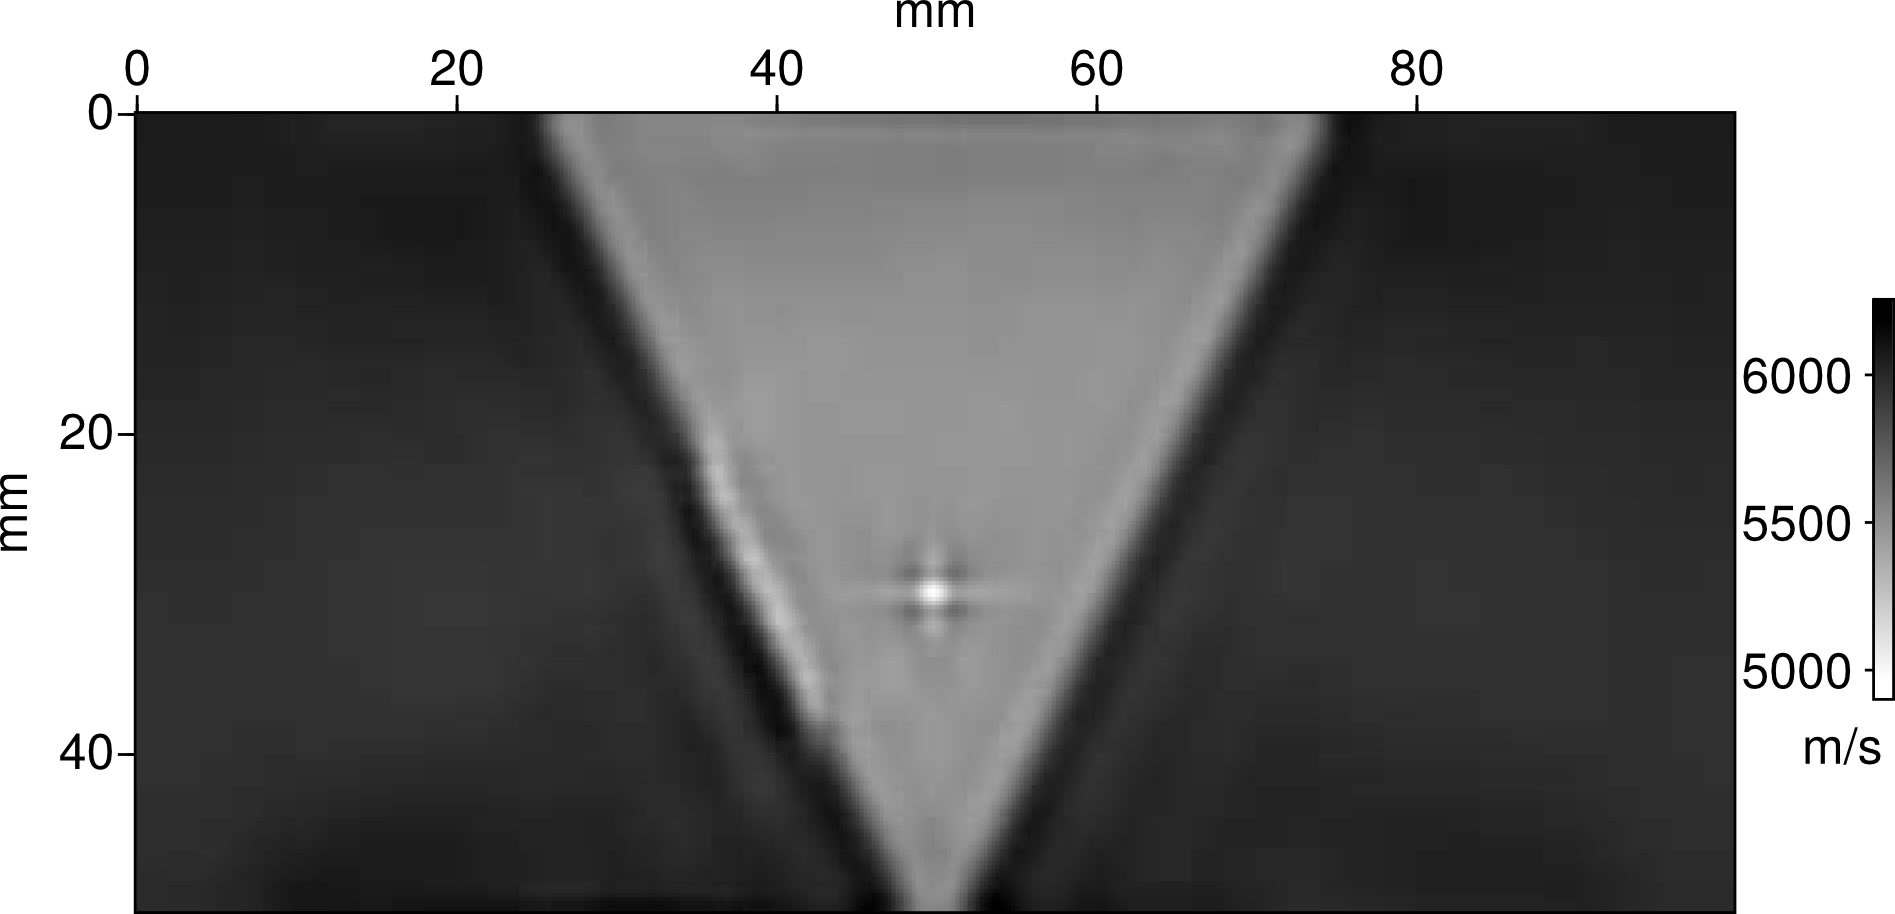
\includegraphics[width=\textwidth]{img/vp_smooth.png}
 		\caption{Vitesse initiale\\~\\}
	\end{subfigure}
    \begin{subfigure}[b]{0.24\textwidth}
 		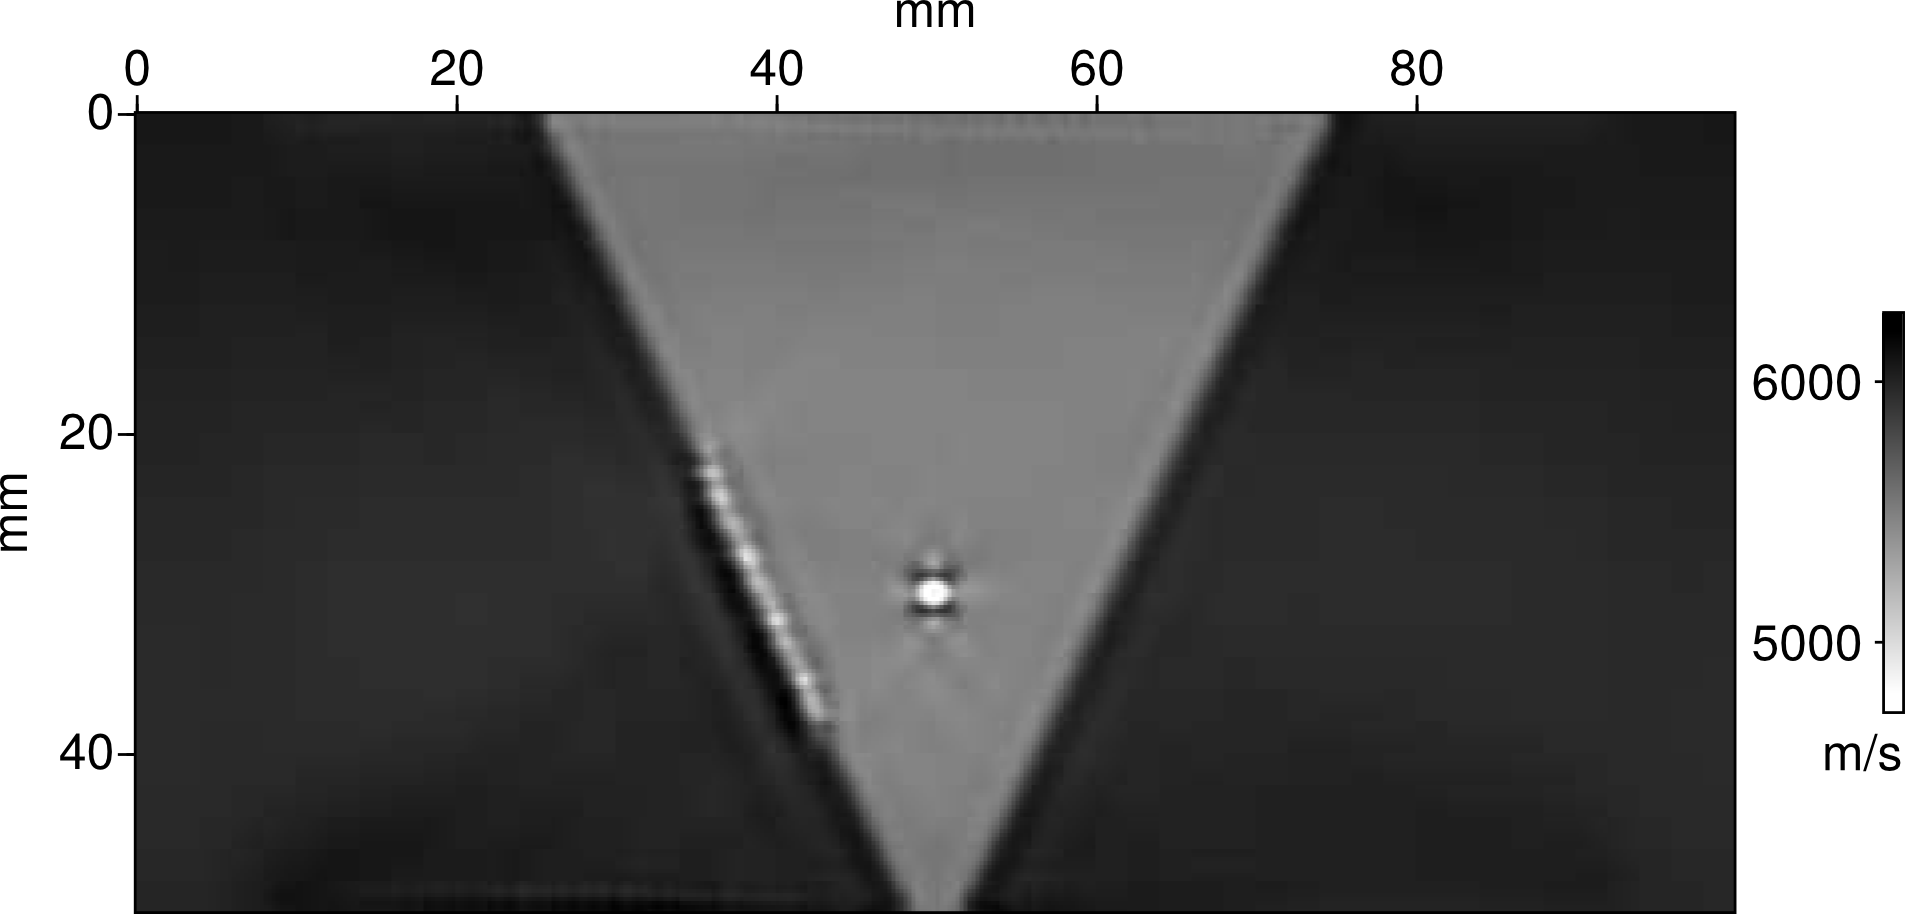
\includegraphics[width=\textwidth]{img/vp_multi_6000k.png}
 		\caption{Vitesse reconstruite par inversion multiparamètre}
	\end{subfigure}
	\begin{subfigure}[b]{0.24\textwidth}
 		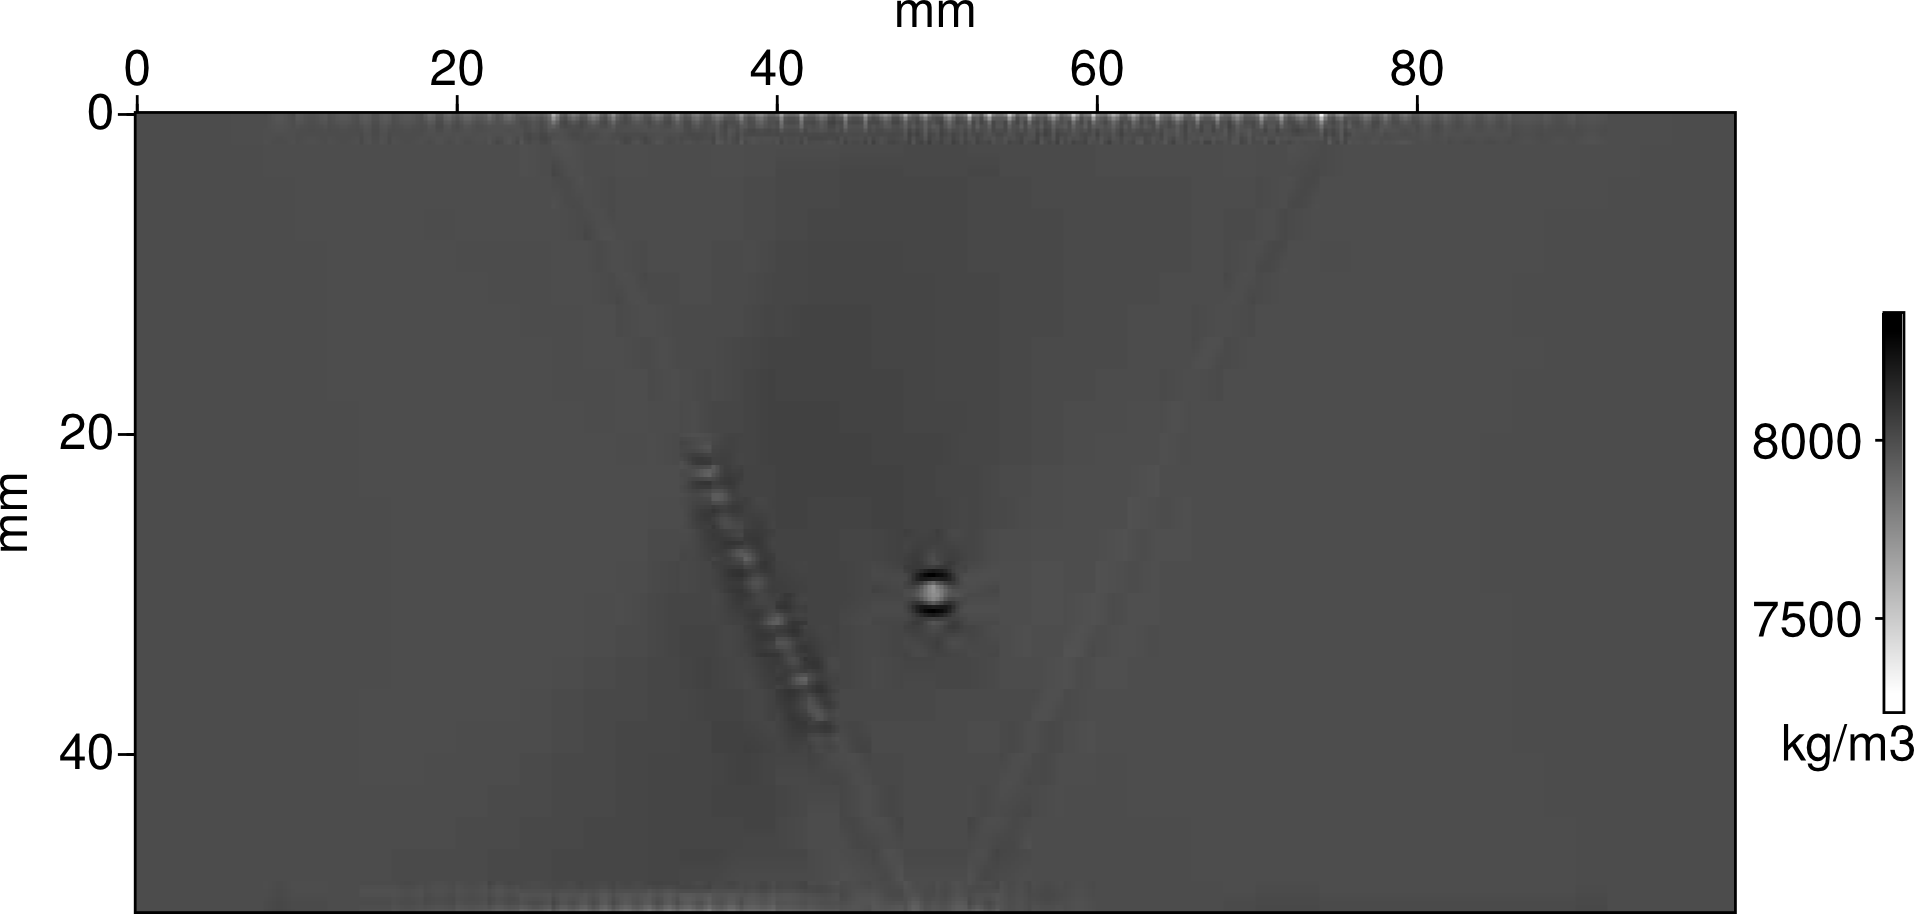
\includegraphics[width=\textwidth]{img/rho_6000k.png}
 		\caption{Masse volumique reconstruite par inversion multiparamètre}
	\end{subfigure}\\
	
	

	\begin{subfigure}[b]{0.3\textwidth}
 		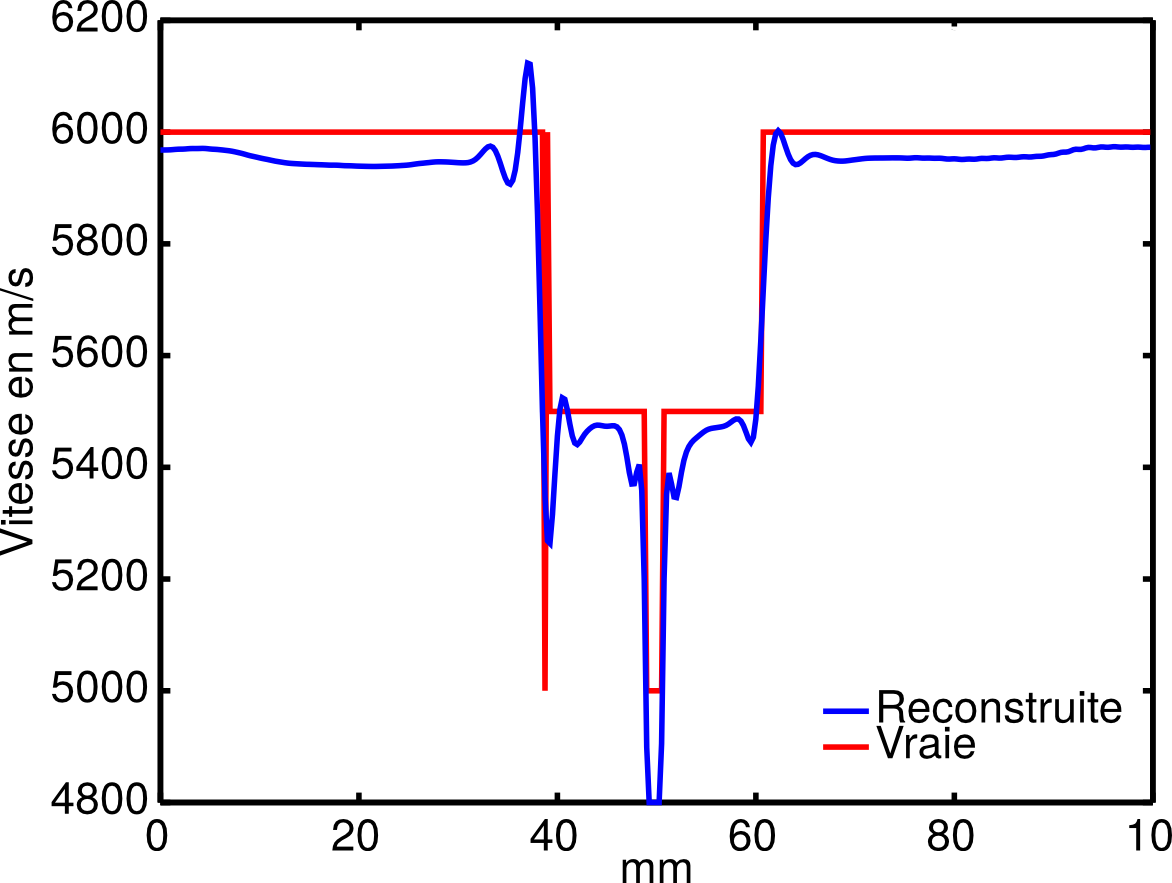
\includegraphics[width=\textwidth]{img/coupe_vp_multi.png}
 		\caption{Coupe en x=5 cm du résultat d'inversion de la vitesse}
	\end{subfigure}
    \begin{subfigure}[b]{0.3\textwidth}
 		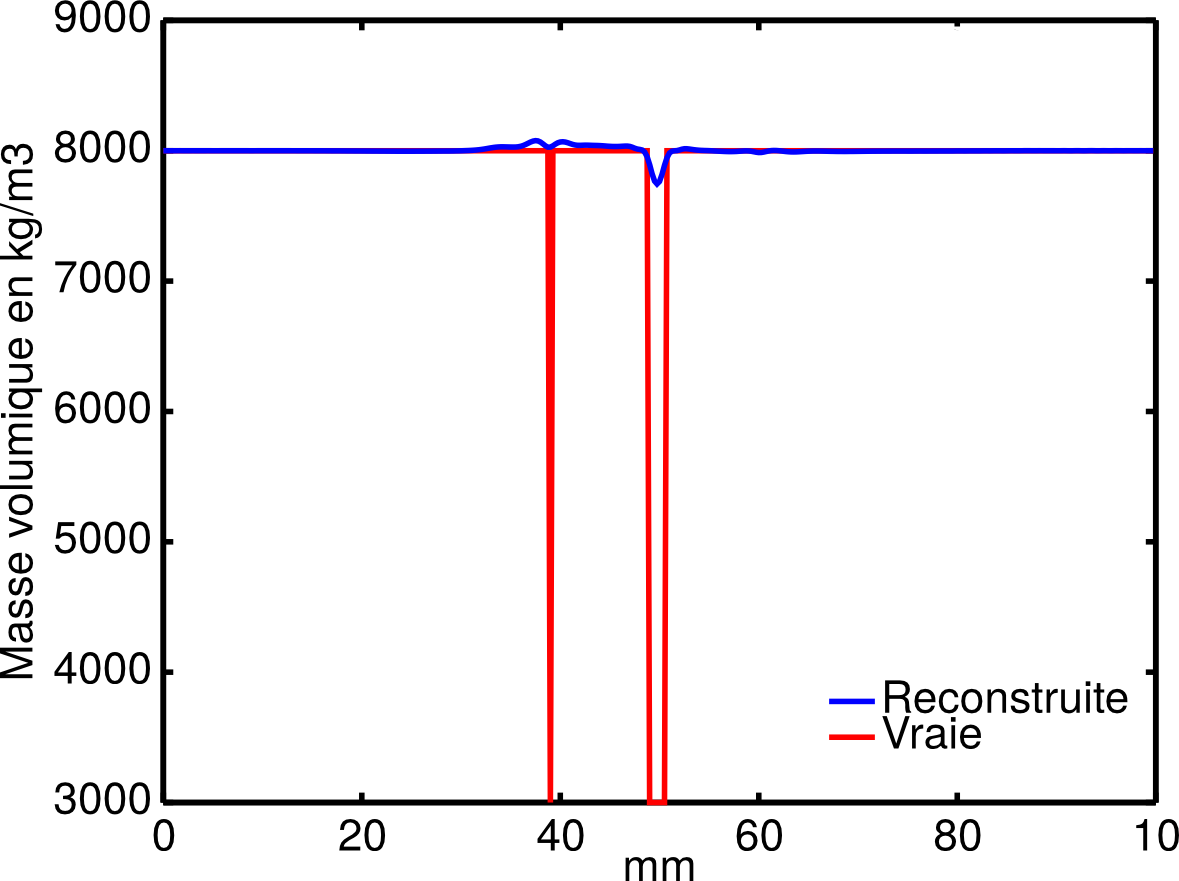
\includegraphics[width=\textwidth]{img/coupe_rho_multi.png}
 		\caption{Coupe en y=3 cm du résultat d'inversion de la masse volumique}
	\end{subfigure}
\end{changemargin}
\end{figure}

\begin{figure}[!h]
\begin{changemargin}{-2cm}{-2cm}
	\centering
    \begin{subfigure}[b]{0.3\textwidth}
 		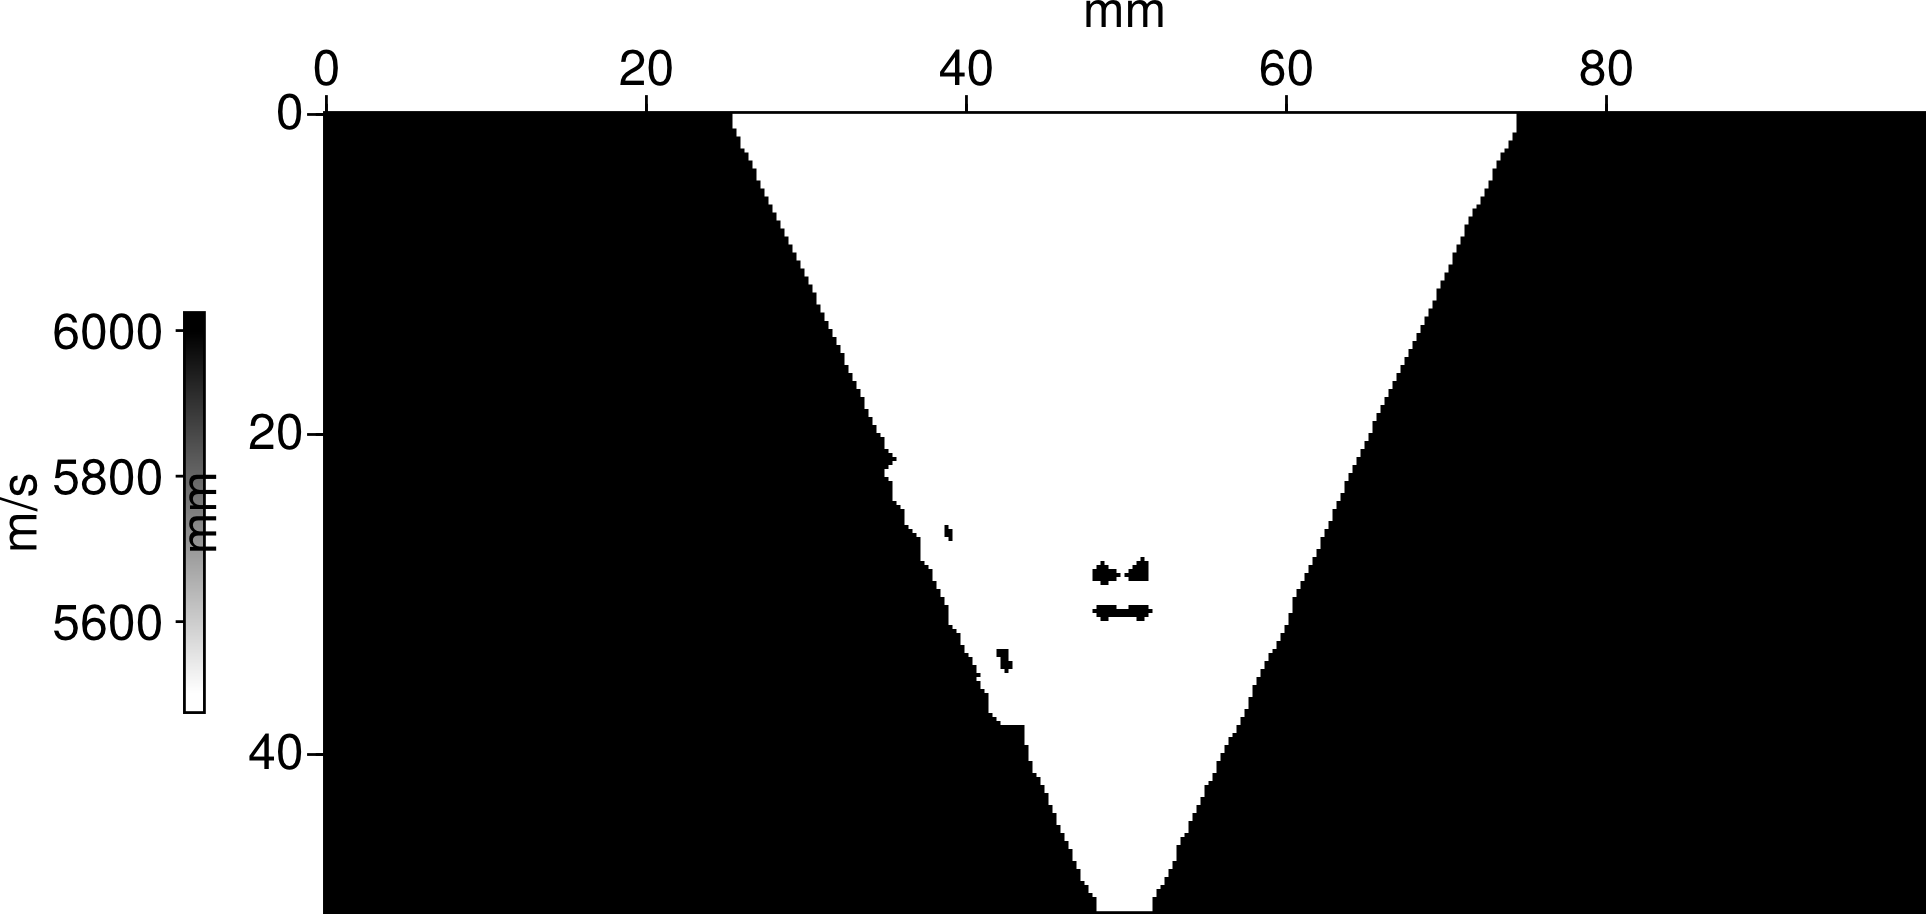
\includegraphics[width=\textwidth]{img/vp_ecrete.png}
 		\caption{Résultat de l'inversion lissée ayant subi un écrêtage}
 	\end{subfigure}
 	\begin{subfigure}[b]{0.3\textwidth}
 		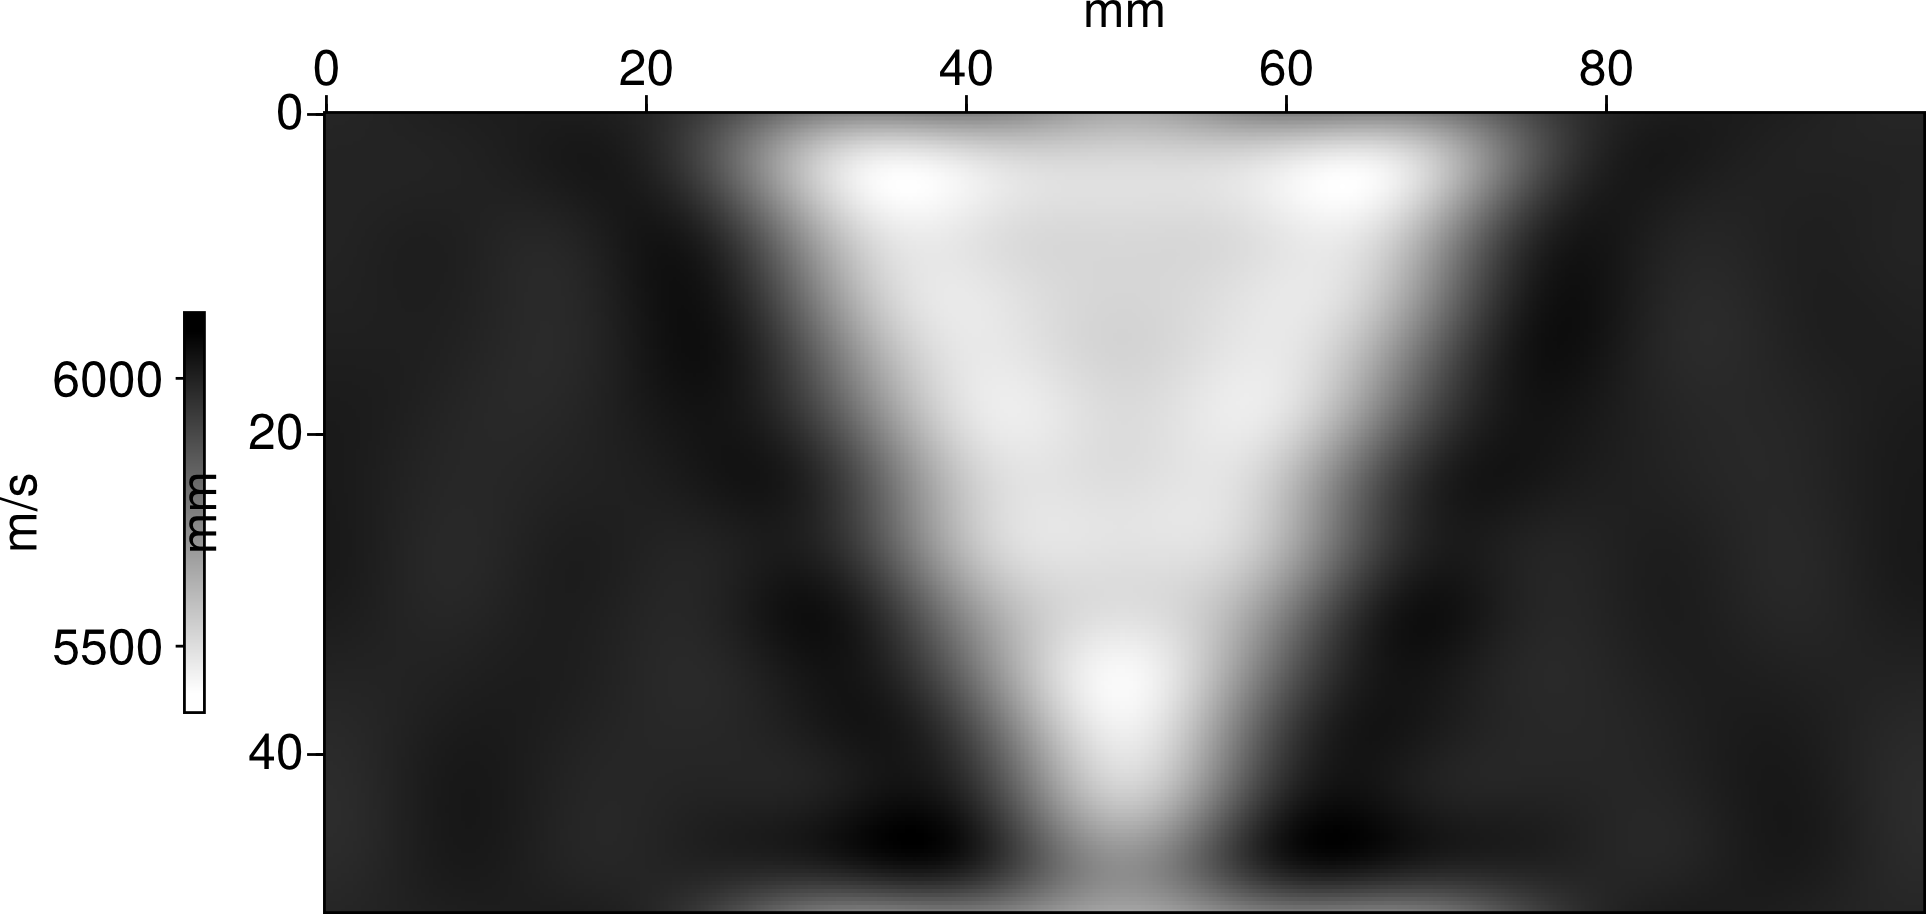
\includegraphics[width=\textwidth]{img/vp_ecrete_filtre.png}
 		\caption{Résultat de l'inversion lissée ayant subi un écrêtage puis un filtrage}
 	\end{subfigure}\begin{subfigure}[b]{0.3\textwidth}
 		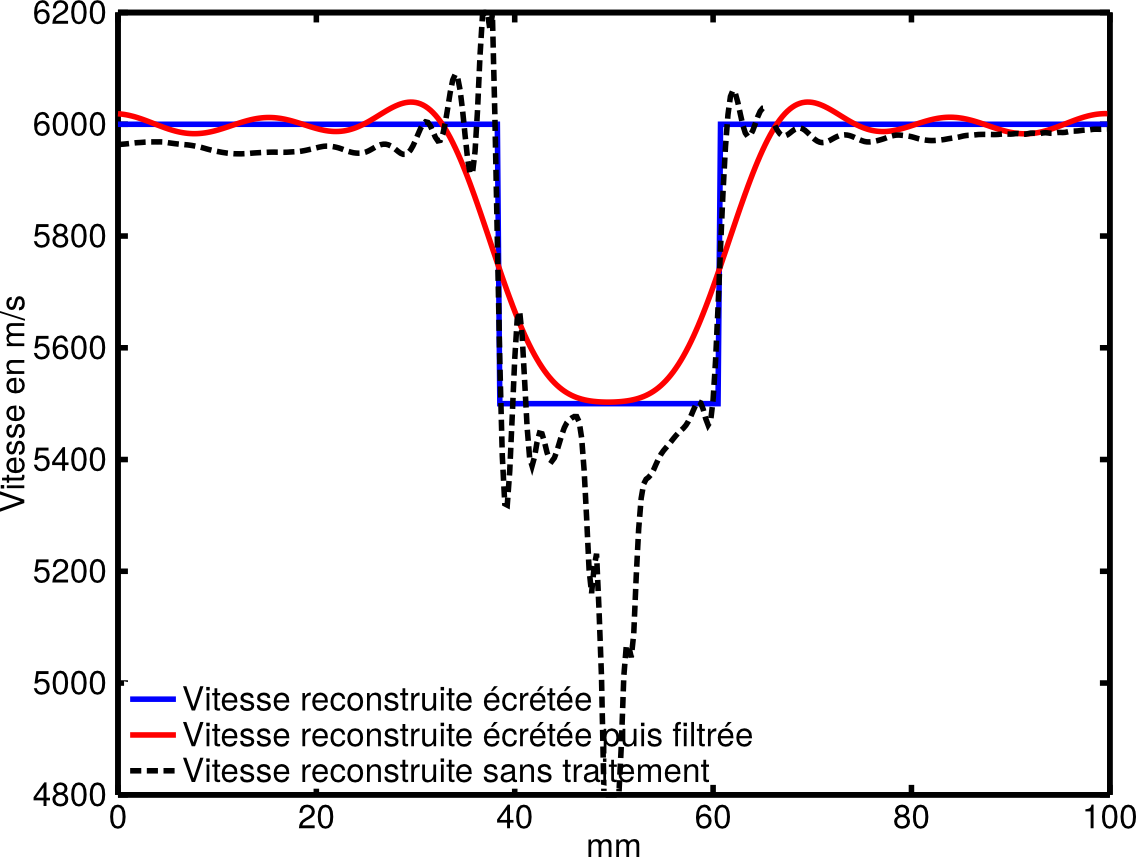
\includegraphics[width=\textwidth]{img/coupe_ecrete_filtre.png}
 		\caption{Coupes à 3 cm de profondeur}
 	\end{subfigure} 
\end{changemargin}	
\end{figure}


À noter que le filtrage bas nombres d'onde réalisé ici ajoute quelques oscillations basses fréquences au modèle.\\

Le modèle initial de masse volumique est toujours uniforme (à 8000 kg/m3). Le résultat de l'inversion multiparamètre réalisée à partir de ce modèle de vitesse écrété-filtré et du modèle de masse volumique homogène est présenté  en figure~\ref{res_ecrete}.

\begin{figure}[!h]
\begin{changemargin}{-2cm}{-2cm}
	\centering
    \begin{subfigure}[b]{0.3\textwidth}
    	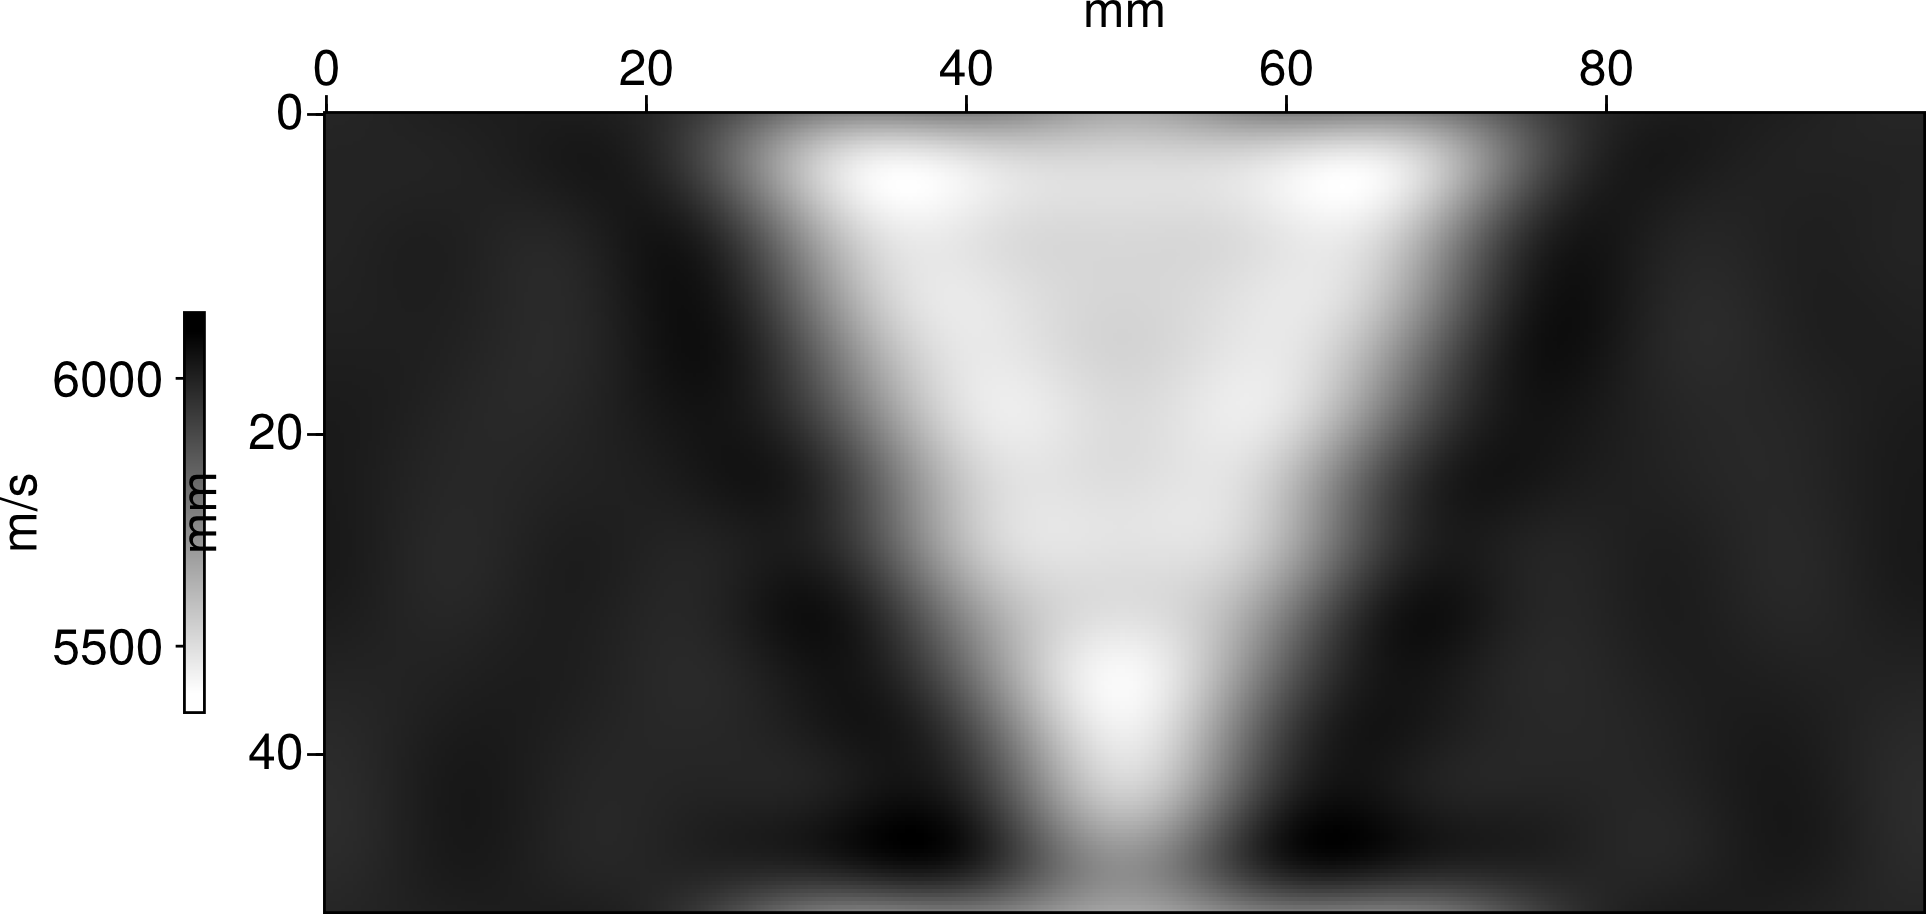
\includegraphics[width=\textwidth]{img/vp_ecrete_filtre.png}
    	\caption{Vitesse initiale\\~}
    \end{subfigure}
    \begin{subfigure}[b]{0.3\textwidth}
    	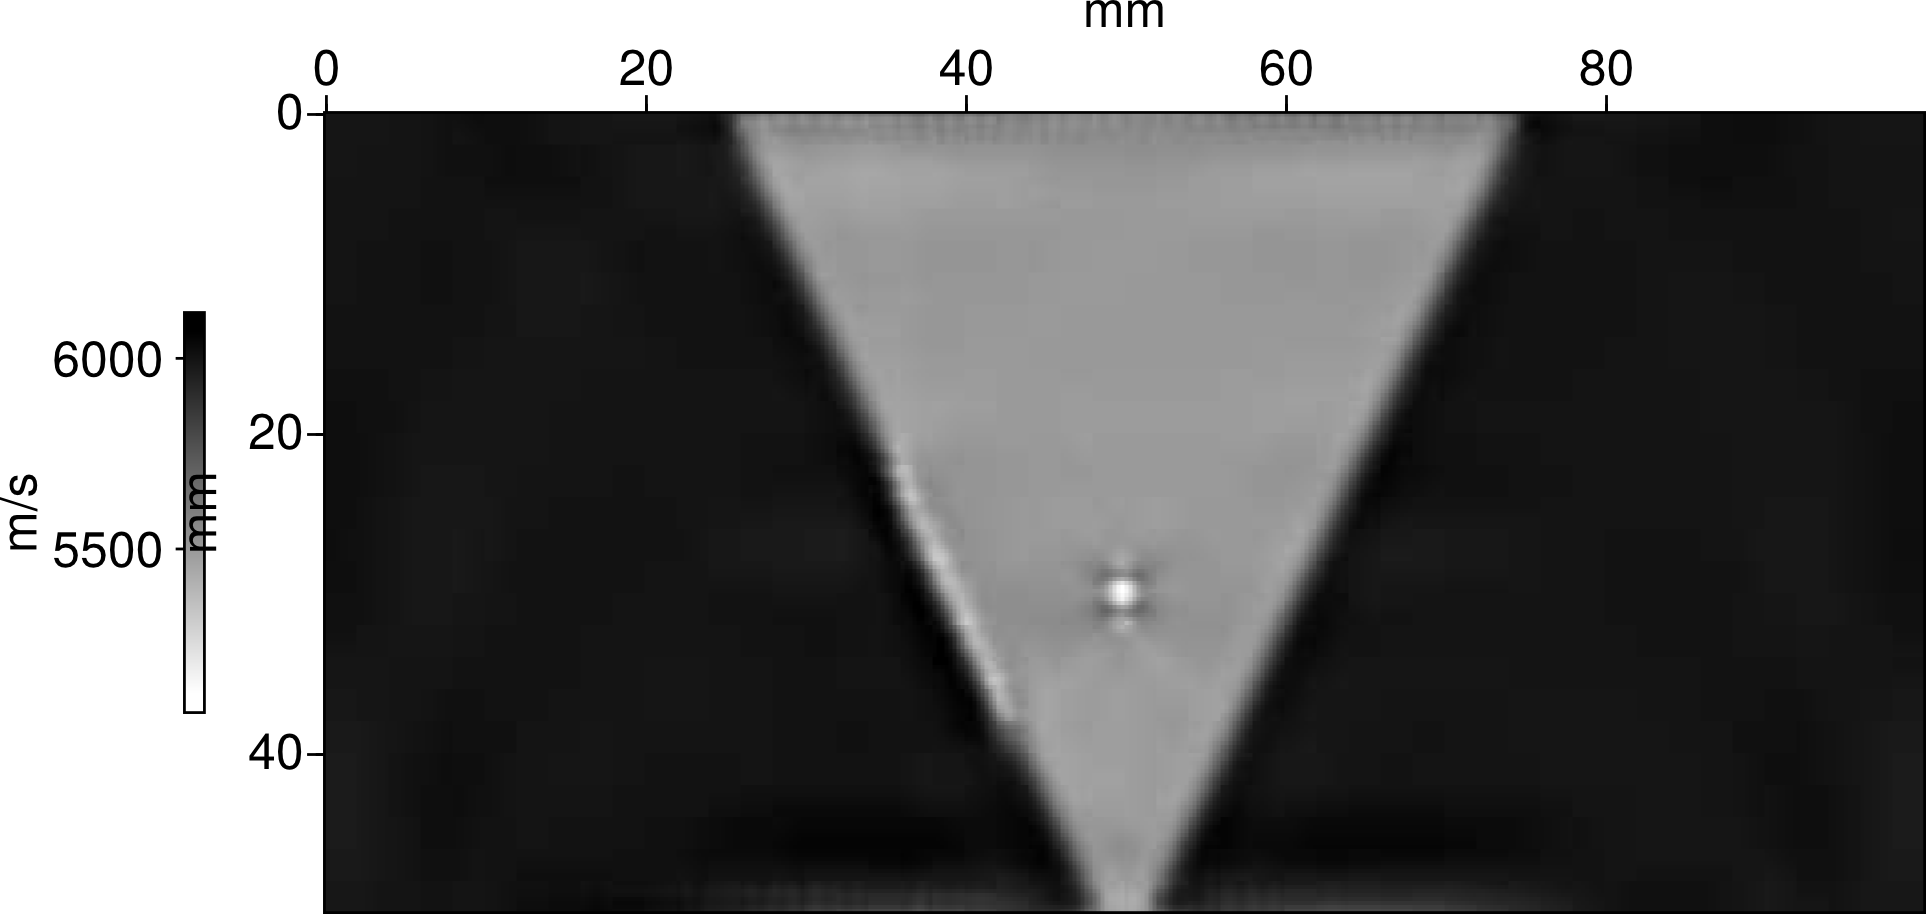
\includegraphics[width=\textwidth]{img/vp_multi_InitEcrete.png}
    	\caption{Vitesse de reconstruite par inversion multiparamètre}
    \end{subfigure}
    \begin{subfigure}[b]{0.3\textwidth}
    	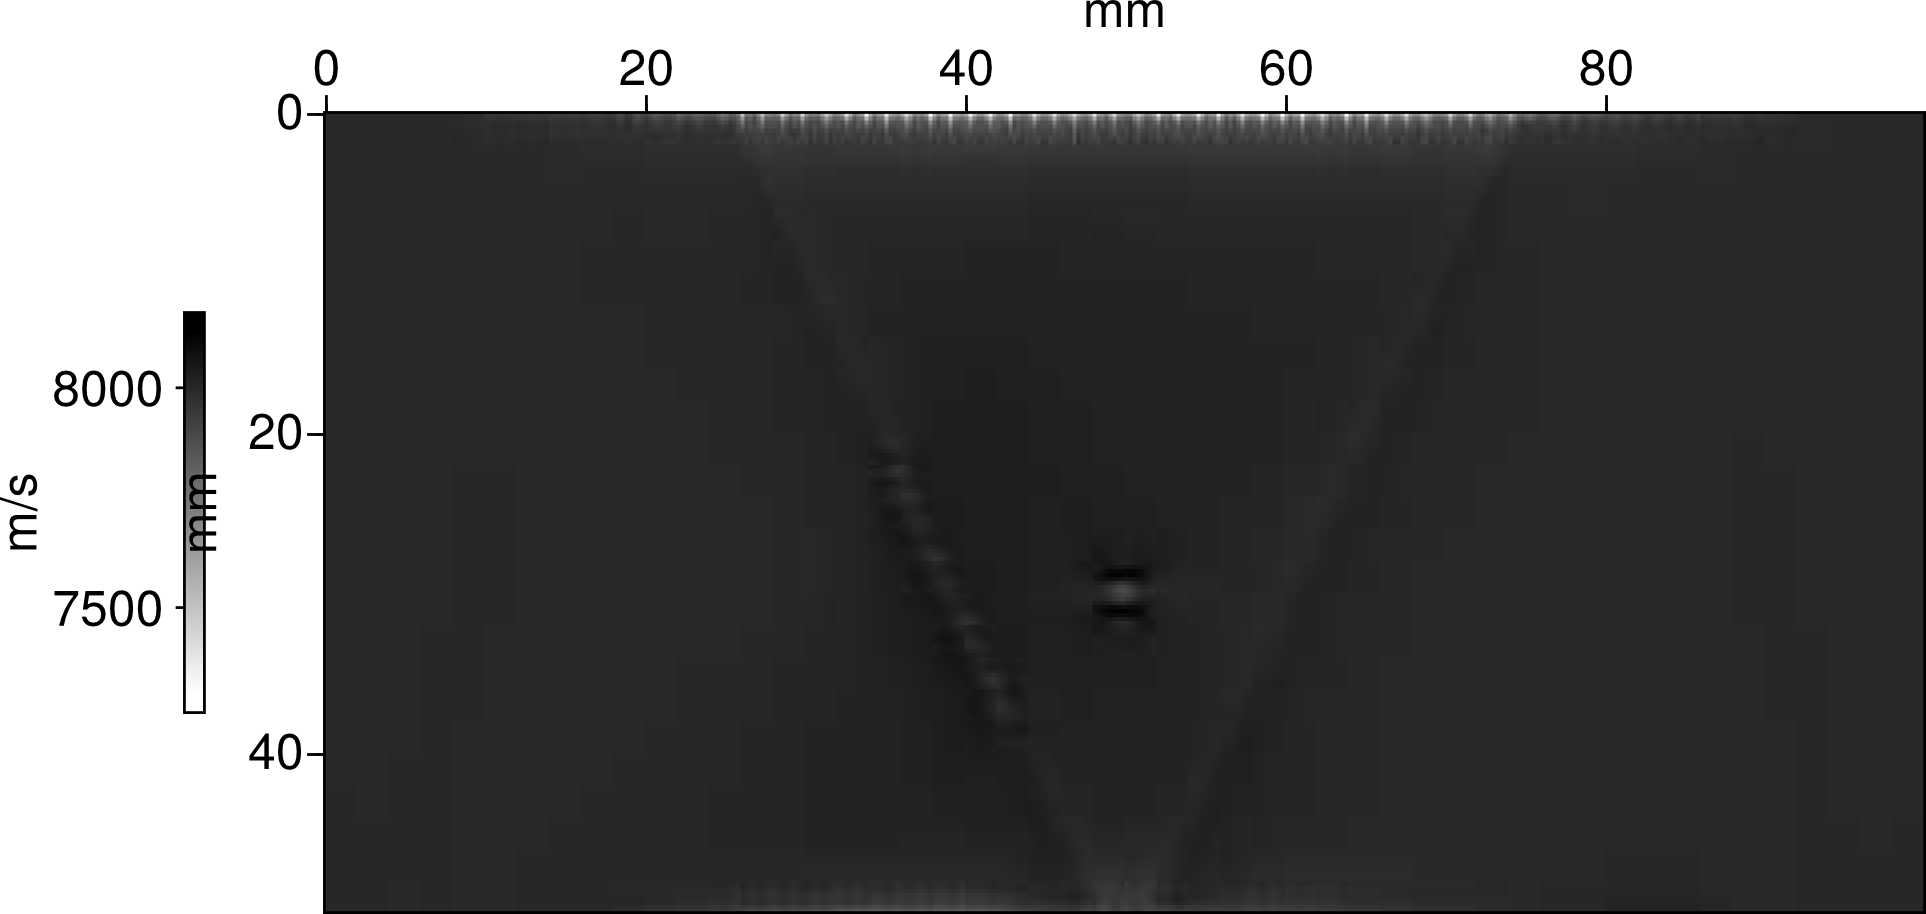
\includegraphics[width=\textwidth]{img/rho_multi_InitEcrete.png}
    	\caption{Masse volumique reconstruite par inversion multiparamètre}
    \end{subfigure}
    
    \begin{subfigure}[b]{0.3\textwidth}
    	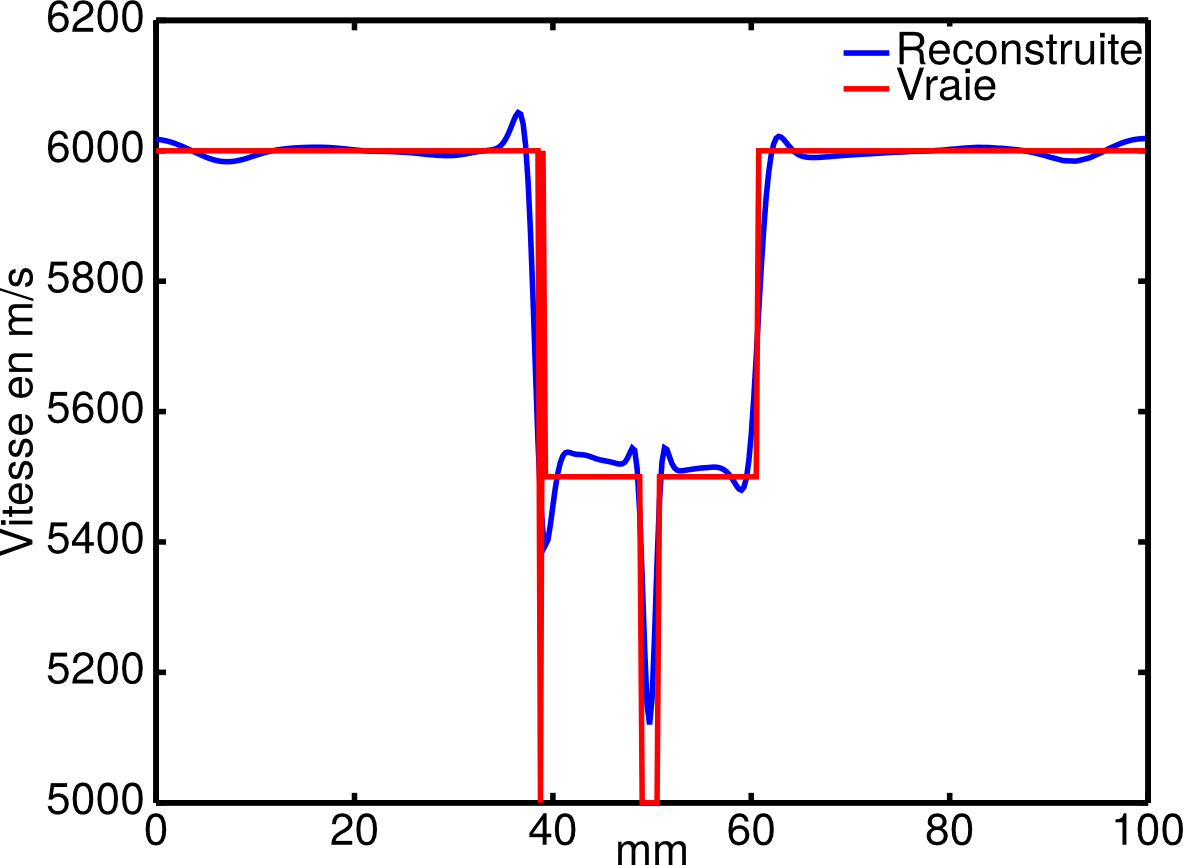
\includegraphics[width=\textwidth]{img/coupe_vp_InitEcrete.png}
    	\caption{Coupe à y = 3 cm de la vitesse reconstruite.}
    \end{subfigure}
    \begin{subfigure}[b]{0.3\textwidth}
    	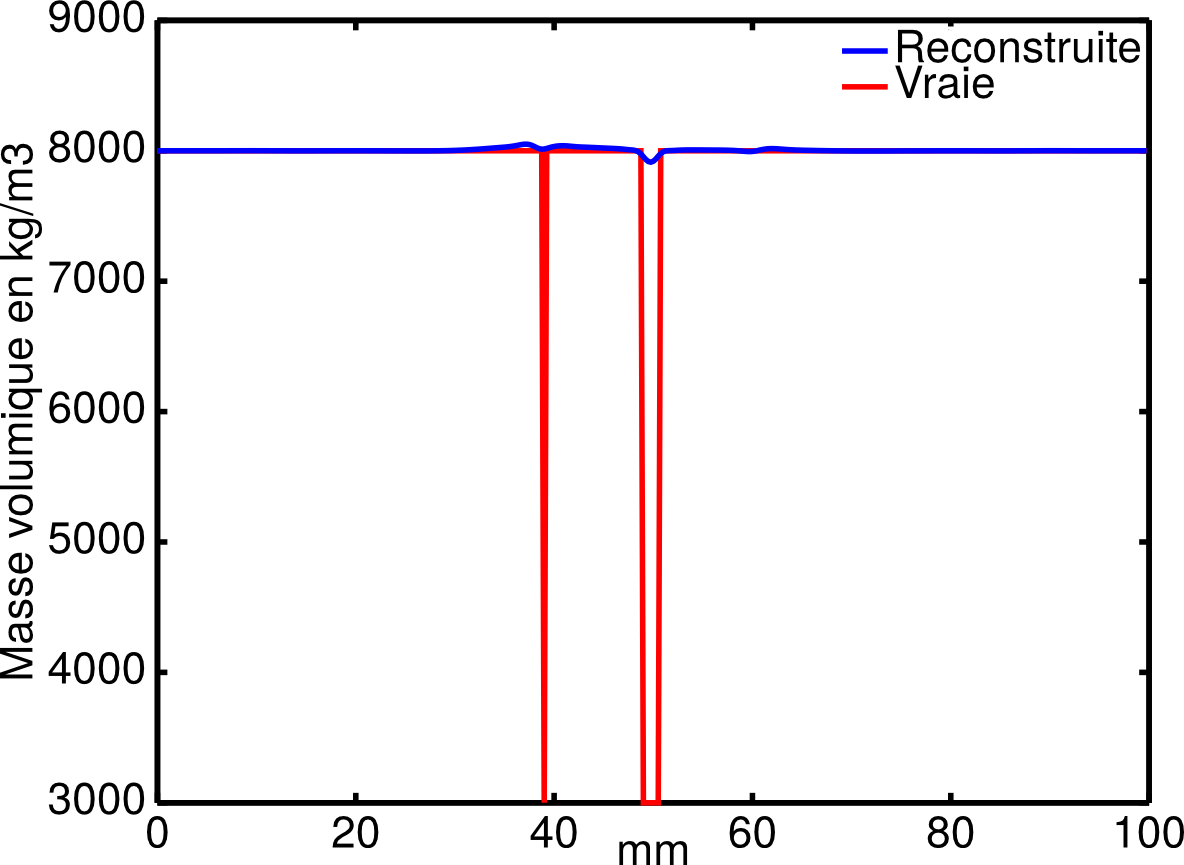
\includegraphics[width=\textwidth]{img/coupe_rho_InitEcrete.png}
    	\caption{Coupe à y = 3 cm de la masse volumique reconstruite.}
    \end{subfigure}
\end{changemargin}
	\caption{\label{res_ecrete}}
\end{figure}

La vitesse ainsi reconstruite est moins perturbée. L'amplitude au niveau des défauts n'est pas toujours pas correcte, mais les bords sont mieux définis. 

 
 
\section{Inversions élastique 3D (SEM3D\_V1.2\_2016\_04)}

Le milieu que l'on cherche à imager est décrit par 3 paramètres : la masse volumique $\rho$, la vitesse des ondes de compression $v_{p}$ et la vitesse des ondes de cisaillement $v_{s}$. La valeur vraie de ces paramètres est données en figure~\ref{milieux_vrais} et dans le tableau~\ref{tab:milieux_vrais} construits sur grille régulière et projeté sur le maillage défini par les noeuds utilisés pour la résolution du problème direct par méthode SEM. Seules des coupes dans le plan (zx) sont représentées ; les milieux sont invariants suivant y .\\

La grille régulière est construite avec : 
\begin{itemize}
	\item nombre de points verticalement : nx=100,
	\item nombre de points horizontalement : nz=200,
	\item nombre de points sur la dimension y : ny=20,
	\item pas de discrétisation (régulier) : h=0.5e-3 m.\\
\end{itemize}

Le maillage SEM a les caractéristiques quivantes : 
\begin{itemize}
	\item 5 noeuds par élément (polynômes d'ordre 4),
	\item sur un élément 1D de longueur unitaire, ces noeuds sont placés aux distances (quadrature de Gauss-Lobatto (?)) : 0 ; 0.17267315 ; 0.5 ; 0.82732685 ; 1,
	\item nelX, le nombre d'élément (non déformés) sur la dimension X,
	\item plusieurs maillages sont utilisés, pour s'adapter à la fréquence des données : \\
	\begin{tabular}{c || c | c | c | c}
						&	nelz	&	nelx	&	nely	&	Largeur des éléments en m (dans toutes les directions) \\ \hline \hline
		Maillage n°1	&	13		&	26		&	3		&	3.85e-3	\\ \hline
		Maillage n°2	&	25		&	50		&	5		&	2e-3	\\ 	
	\end{tabular}
\end{itemize}

Temporellement, les signaux sont acquis sur 32 $\mu$s, soit 4000 points avec un échantillonnage de 8e-9 s. L'acquisition est composées de 2 barrettes 64 éléments placées de part et d'autre de la soudure. Celle du haut est utilisée en excitation, celle du bas en transmission.


\begin{figure}[!h]
	\begin{changemargin}{-2cm}{-2cm}
		\begin{subfigure}[b]{0.3\textwidth}
			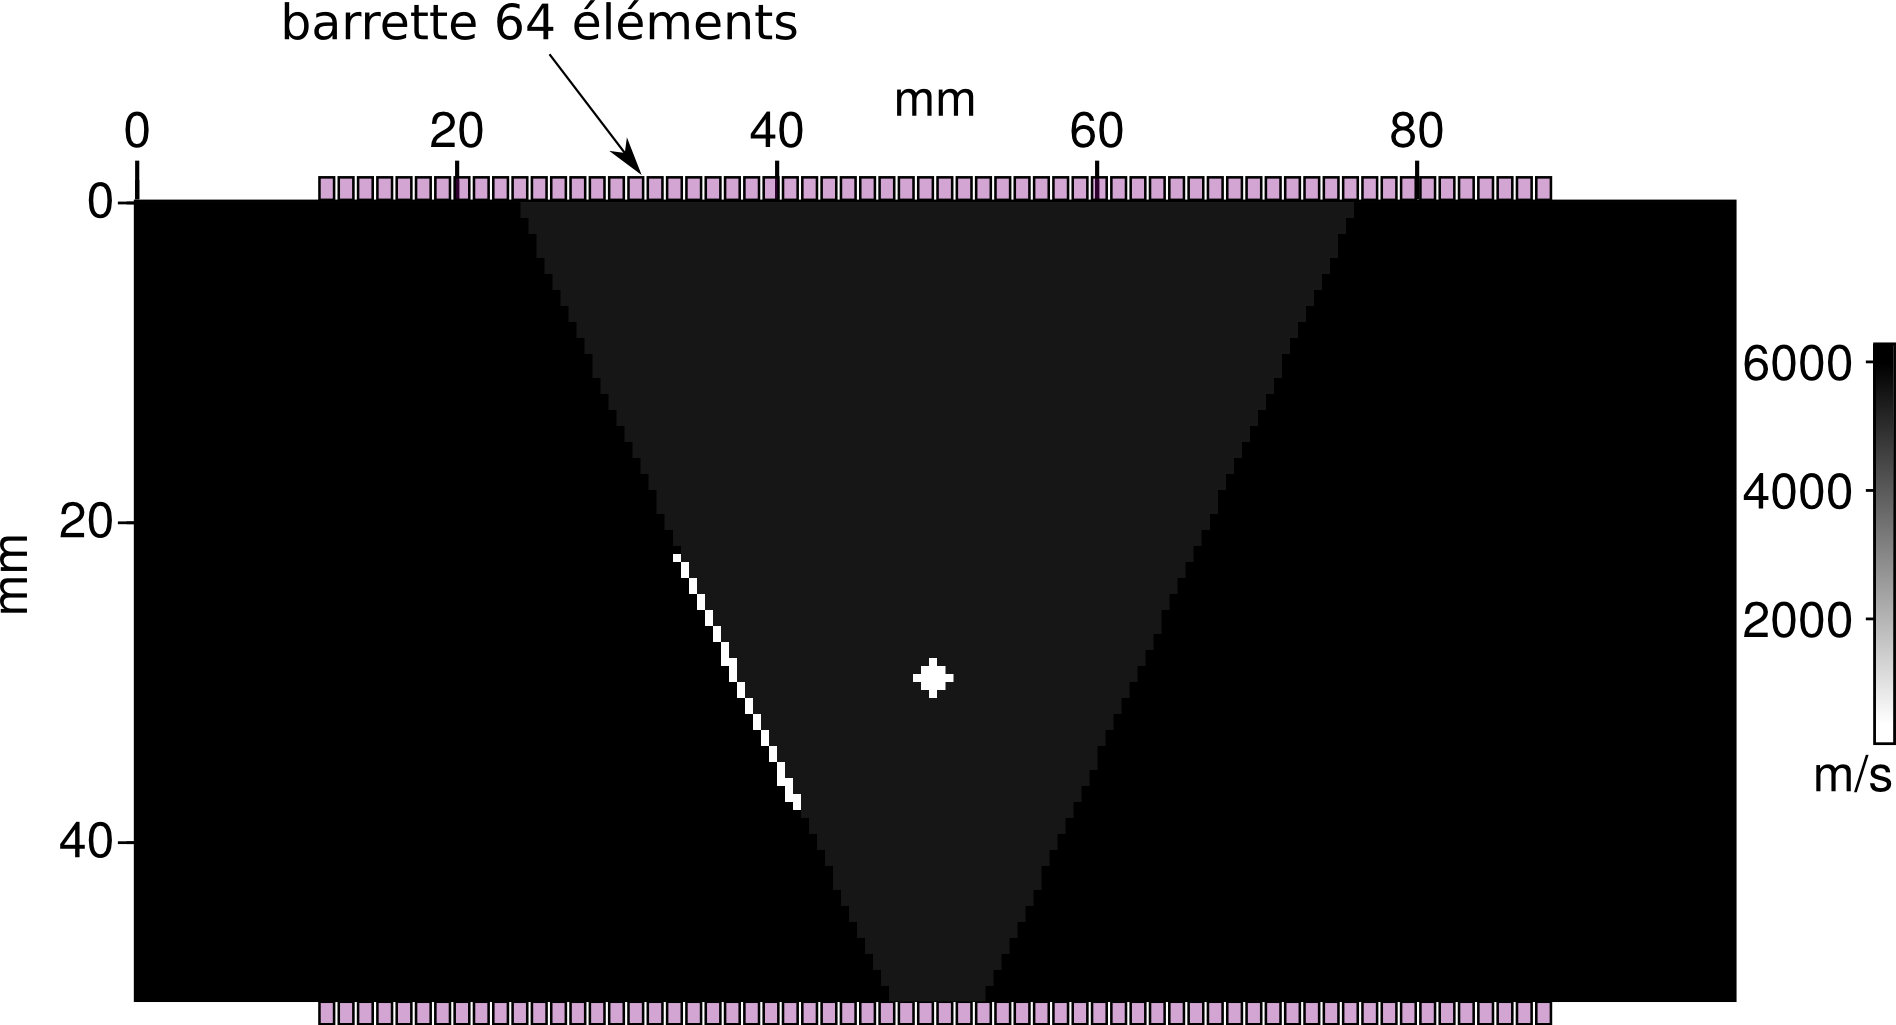
\includegraphics[width=\textwidth]{img/vp_true_reg.png}
			\caption{$v_{p}$ vrai}
		\end{subfigure}
		\begin{subfigure}[b]{0.3\textwidth}
			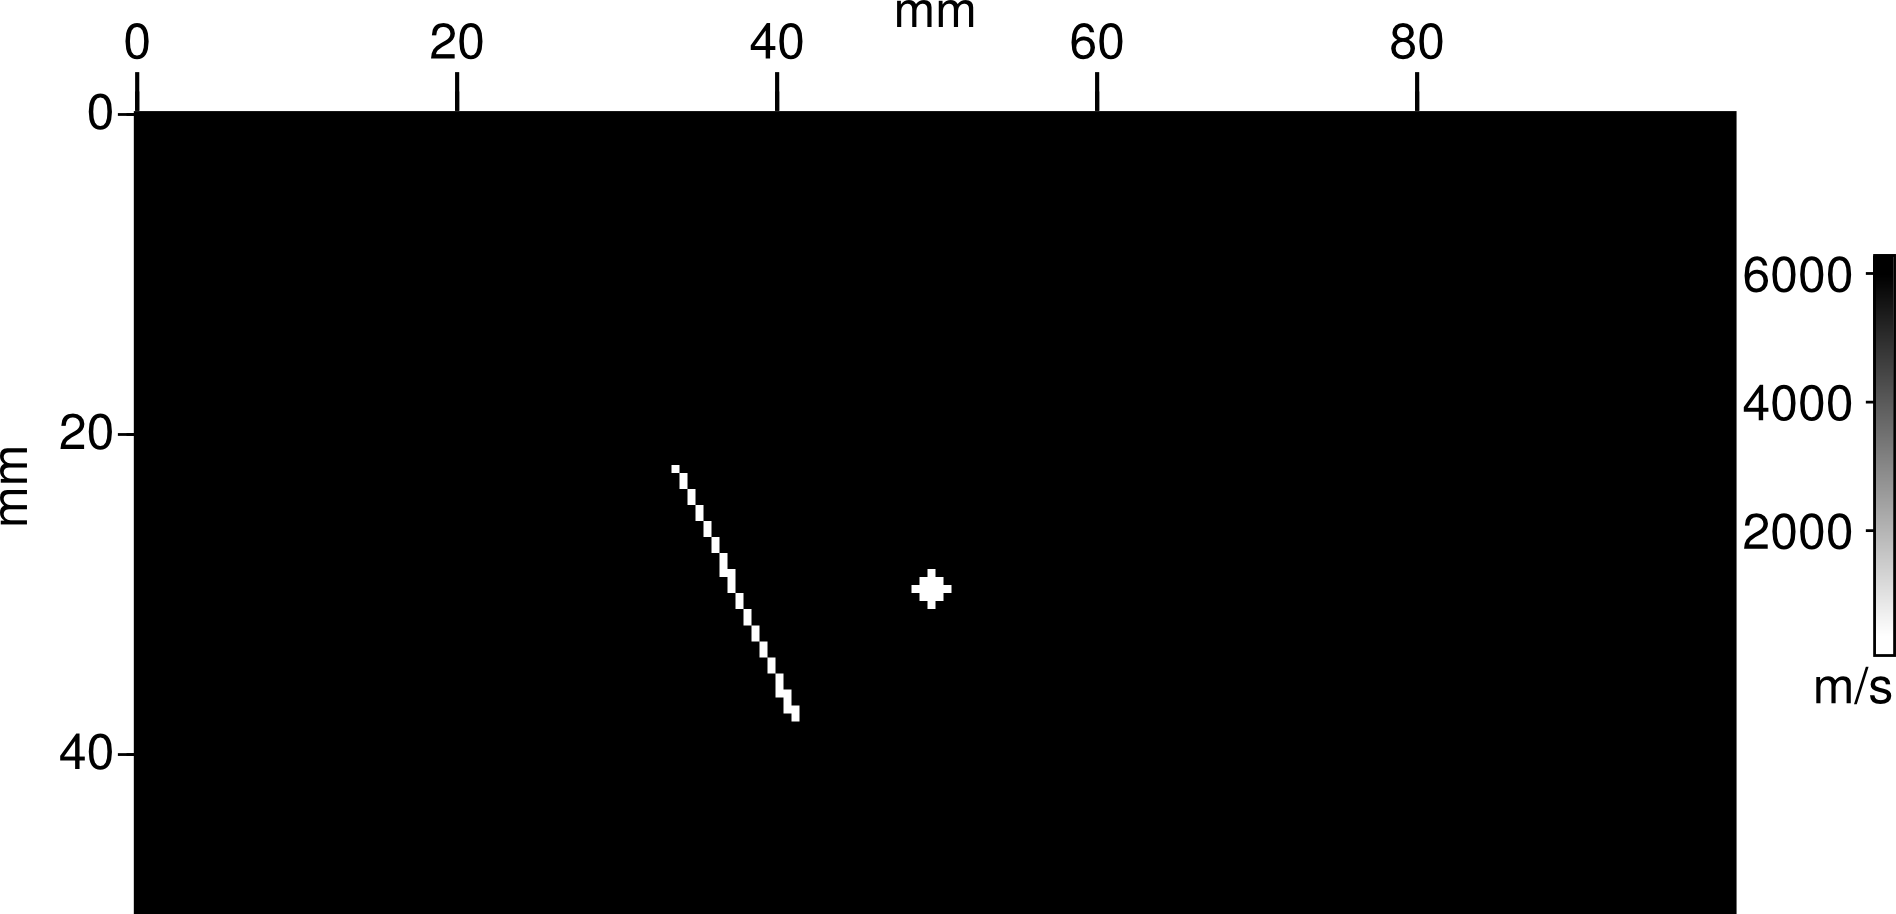
\includegraphics[width=\textwidth]{img/vs_true_reg.png}
			\caption{$v_{s}$ vrai}
		\end{subfigure}
		\begin{subfigure}[b]{0.3\textwidth}
			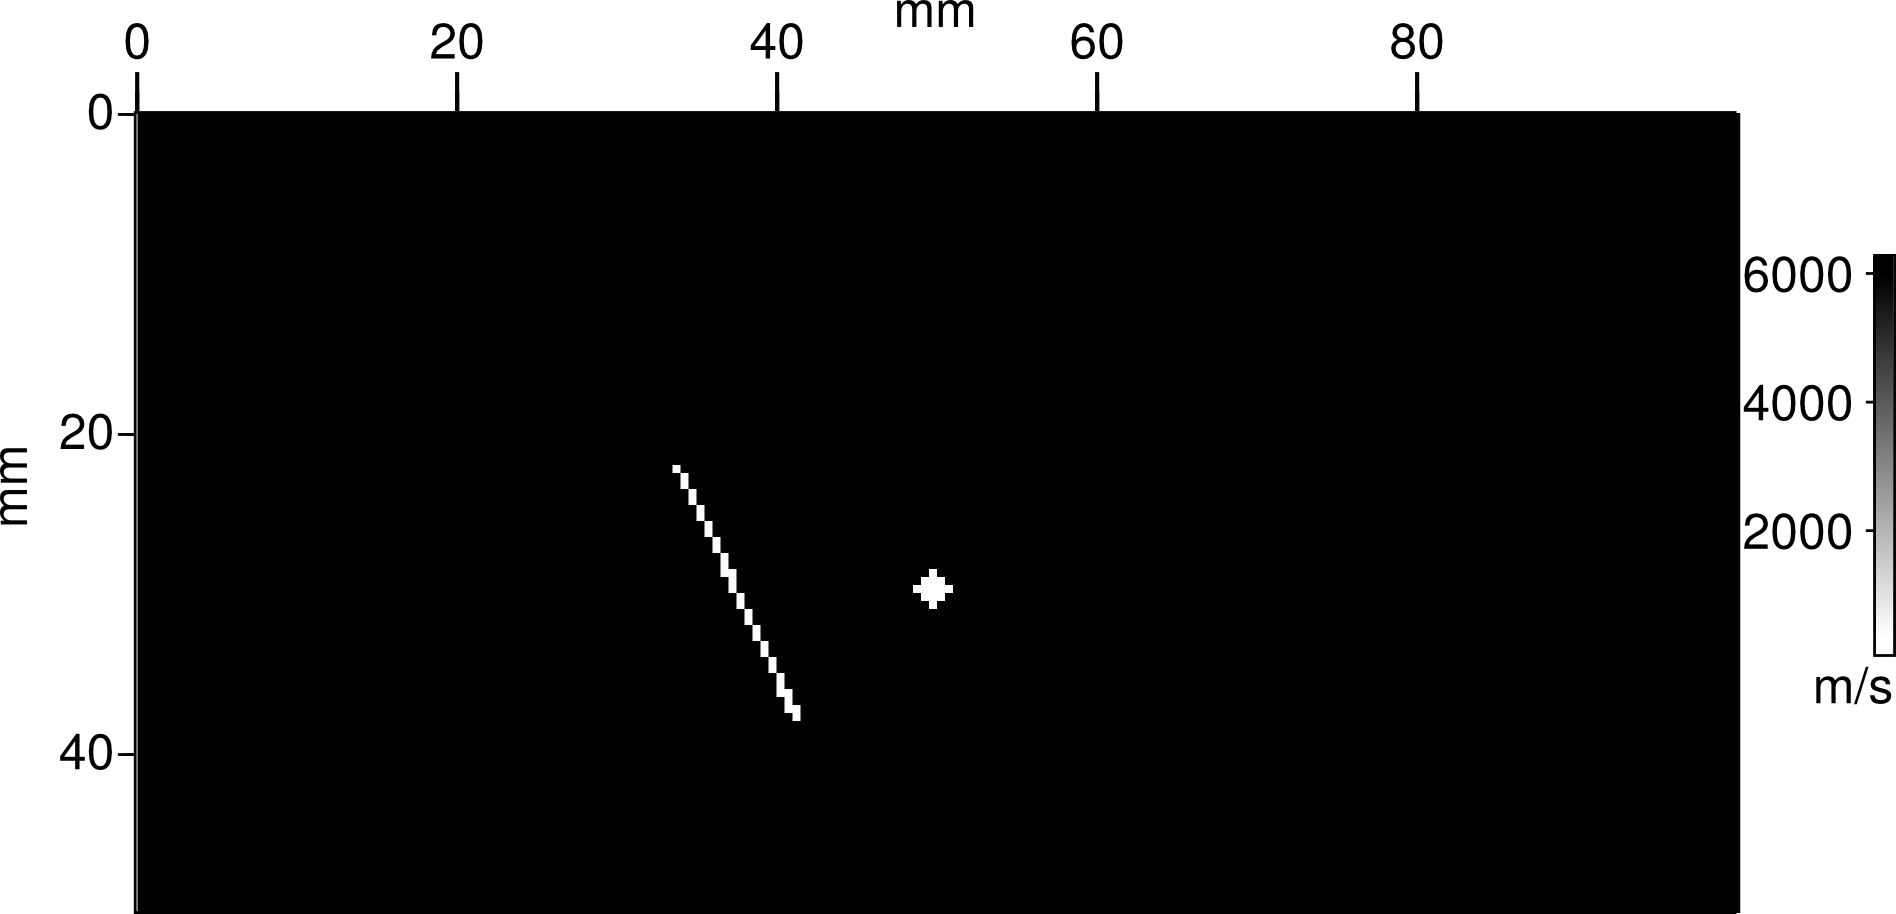
\includegraphics[width=\textwidth]{img/rho_true_reg.png}
			\caption{$\rho$ vrai}
		\end{subfigure}\\
		
		\begin{subfigure}[b]{0.3\textwidth}
			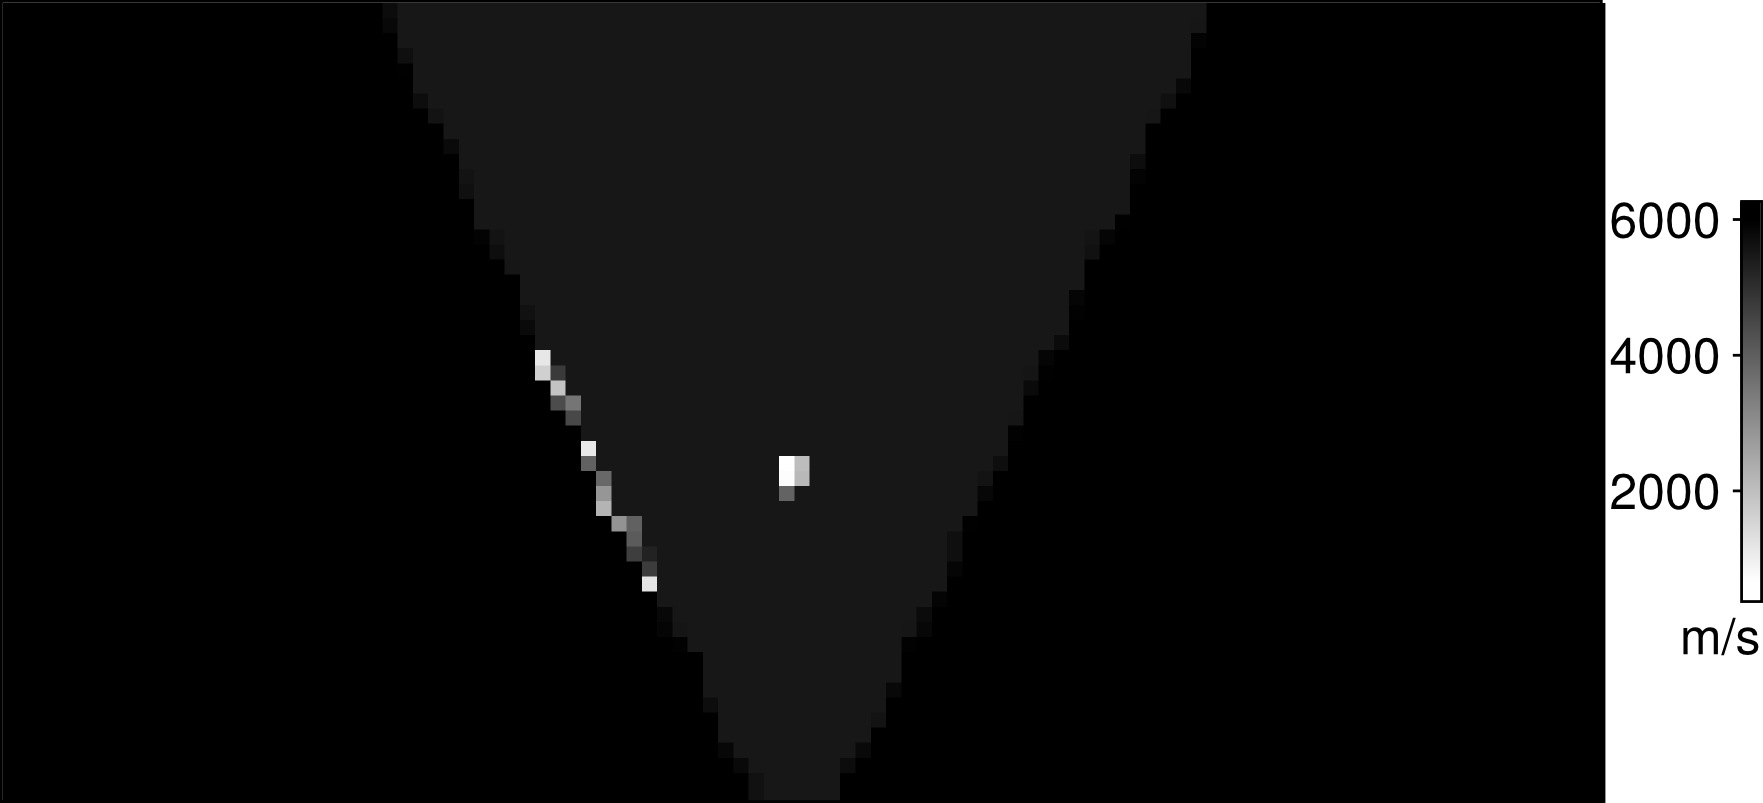
\includegraphics[width=\textwidth]{img/vpfile.png}
			\caption{$v_{p}$ vrai}
		\end{subfigure}
		\begin{subfigure}[b]{0.3\textwidth}
			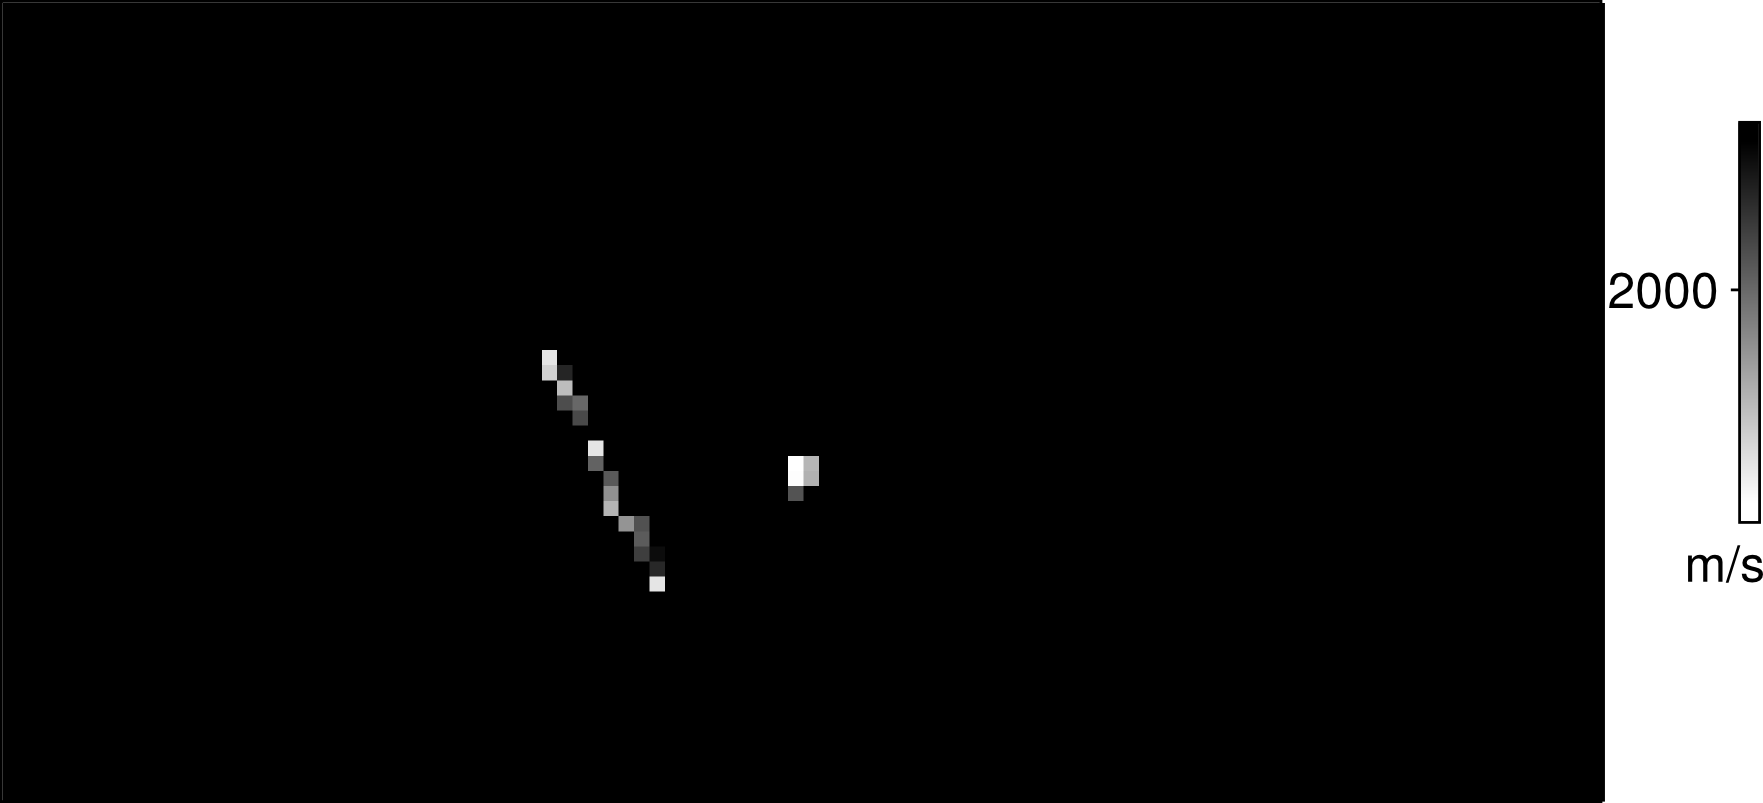
\includegraphics[width=\textwidth]{img/vsfile.png}
			\caption{$v_{s}$ vrai}
		\end{subfigure}
		\begin{subfigure}[b]{0.3\textwidth}
			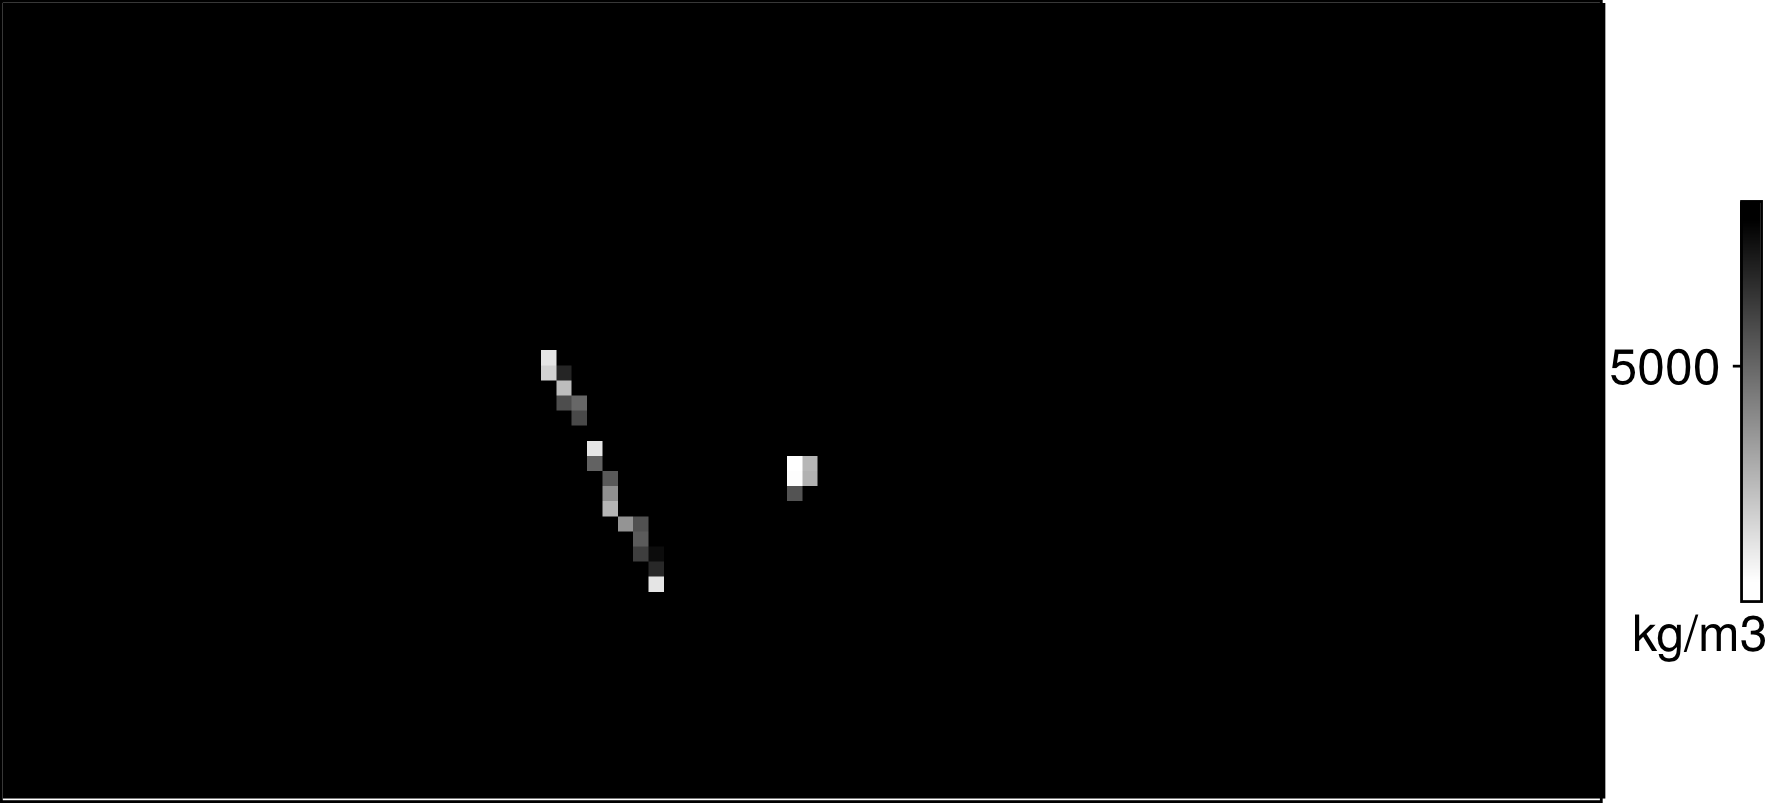
\includegraphics[width=\textwidth]{img/rhofile.png}
			\caption{$\rho$ vrai}
		\end{subfigure}
	\end{changemargin}
	\caption{\label{milieux_vrais}Milieux vrais sur grille régulière (en haut) et interpolé sur les éléments SEM (en bas). L'acquisition est composées de 2 barrettes 64 éléments placées de part et d'autre de la soudure. Celle du haut est utilisée en excitation, celle du bas en transmission.}
\end{figure}

\begin{table}[!h]
	\centering
	\begin{tabular}{c || c | c | c}
										& $v_{p}$ (m/s) & $v_{s}$ (m/s) & $\rho$ (kg/m$^3$)\\ \hline \hline
								Plaque  & 6000  		& 3200 			& 8000 \\ \hline
								Soudure & 5500			& 3200 			& 8000 \\ \hline
		Défauts sur grille régulière 	& 340			& 100			& 100	\\ \hline
Défauts sur grille SEM 	(valeurs min.)	& 636			& 277			& 553 \\ 

	\end{tabular}
	\caption{Valeurs des paramètres dans différentes zones. \label{tab:milieux_vrais}}
\end{table}


Une modification est apportée à la routine \emph{modeling\_fwi.f90} de manière à ce que le gradient soit rendu invariant suivant y, à sa valeur moyenné sur l'ensemble des coupes en y : 

\begin{changemargin}{-2cm}{-2cm}
\noindent \begin{small}	
	\begin{verbatim}
	    DO ipar=1,inv%npar
	        DO i3=1,pbdir%nddl3_glob
	            inv%gradient_glob(:,:,i3,ipar)=sum(inv%gradient_glob(:,:,:,ipar),dim=3)/pbdir%nddl3_glob
	        END DO	 
	    END DO
	\end{verbatim}
\end{small}
\end{changemargin}

De plus, le filtre médian est appelé jusqu'à 3 fois (en basses fréquences), de manière à réduire les perturbations hautes fréquences du gradient.


\subsection{Fixer les bornes}
 
Le coefficient de Poisson est tel que : 
\begin{equation}
	v_{p} = \sqrt{\frac{2(1-\mu)}{(1-2)}} v_{s}~~~~~	\Leftrightarrow~~~~~  \mu = \frac{2v_{s}^2-v_{p}^2}{2v_{s}^2-2v_{p}^2}.
\end{equation}
On souhaite qu'en tout point du milieu, le coefficient de Poisson reste positif. Comme $v_{p}>v_{s}$, il faut que : 
\begin{equation}
	2v_{s}^2 - v_{p}^2 <0 ~~~~~\Leftrightarrow~~~~~ v_{s}< \frac{v_{p}}{sqrt(2)}. \label{poisson}
\end{equation}

Les bornes du milieu sont donc à fixer en conséquence, de manière à bien contraindre l'inversion à respecter cette relation. Plusieurs stratégies peuvent être mises en place.

\subsection{Génération des données}

L'inversion à partir de données HF filtrées donne de fortes singularités au niveau des sources et des récepteurs. Elles sont peut-être dues à l'absence de pré-conditionnement du Hessien (amélioration en cours de développement ?). Pour éviter ces singularités, les données ne sont pas filtrées mais regénérées pour chaque inversion dans une nouvelle bande de fréquence. L'excitation et le maillaige utilisés pour l'inversion sont les mêmes que ceux utilisés pour la génération des données.

\begin{figure}[!h]
	\centering
	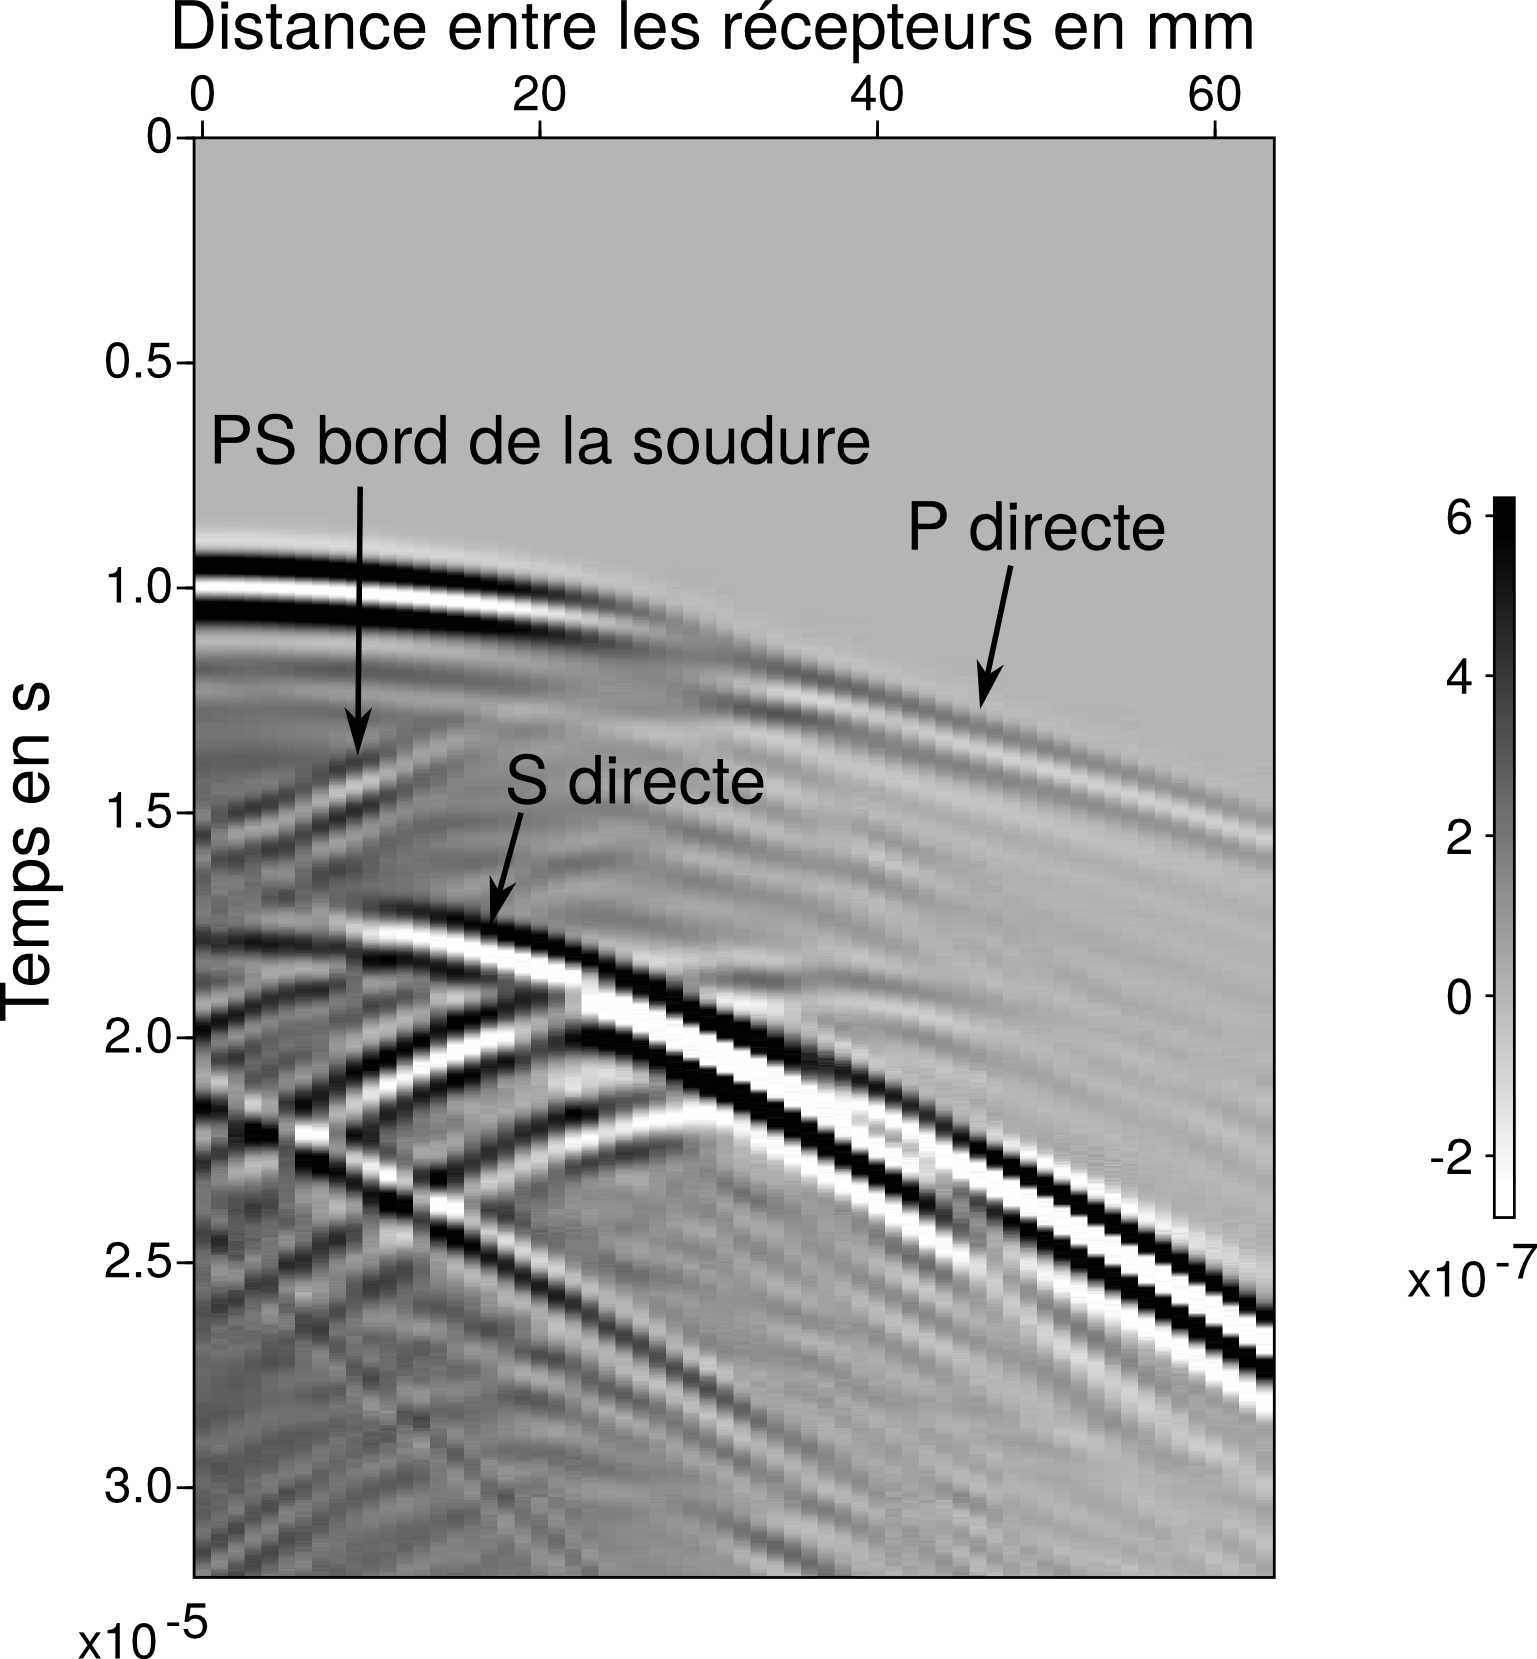
\includegraphics[height=5cm]{img/multi_trans/data_750k.png}
	\caption{Données observées pour une excitation à 750 kHz.\label{data_obs}}

\end{figure}

\subsection{Stratégies d'inversion}


\subsubsection{Inversions monoparamètres}
Les ondes de compression et de cisaillement ont une empreinte du même ordre de grandeur sur les données observées (cf figure~\ref{data_obs}). Il est donc indispensable de pondérer les données avant une inversion monoparamètre ($v_{p}$ ne doit pas être reconstruit par interprétation des ondes S, par exemple).

\subsubsection{Inversions multiparamètres}

L'inversion multiparamètre ne demande pas de pré-traitement des données mais nécessite de contraindre l'inversion pour que la condition~\ref{poisson} soit respectée. Pour cela, il est possible de fixer les valeurs limites que peuvent prendre les différents paramètres. Ces bornes peuvent être définies globalement (pour l'ensemble du milieu) ou localement (en chaque point du milieu). Comme les zones susceptibles de poser problèmes sont celles des défauts et que ces zones sont considérées inconnues, on doit définir les bornes globalement. Suite aux résultats des inversions basses fréquences, les défauts seront globalement localisés et en cas de problème avec la condition~\ref{poisson}, il sera possible de définir d'autres bornes dans ces zones.\\

Les valeurs des bornes globales pour chaque bande de fréquence sont données dans le tableau~\ref{tab:bornes}.

\begin{table}[!h]
\begin{changemargin}{-2cm}{-2cm}
	\begin{tabular}{c || c | c || c | c || c || c}
		Gamme de fréquence	& $v_{{p}_{min}}$	& $v_{{p}_{max}}$	 & $v_{{s}_{min}}$	 & $v_{{s}_{max}}$	 & Nombre de filtres médians appliqués &  Maillage SEM \\ \hline \hline
		150 kHz				& 5000				& 6500				& 1000				& 3200				& 3 	&	Maillage n°1\\ \hline		
		225 kHz				& "					& " 				& "					& "					& " 	&	Maillage n°1 \\ \hline
		337 kHz				& "					& " 				& "					& "					& " 	&	Maillage n°1 \\ \hline
		337 kHz				& 3500 				&	6500			&	100				& 3200				& 2 	&	Maillage n°1 \\ \hline
		500 kHz				& 3500 				&	6500			&	100				& 3200				& 1 (donne un gradient trop crénelé) 	&	Maillage n°1 \\ \hline
		750 kHz				& "					& " 				& "					& "					& 2 	&	Maillage n°2 \\ \hline
		1 MHz				& "					& " 				& "					& "					& " 	&	Maillage n°2 \\ \hline
	\end{tabular}
	\caption{Bornes, nombre de filtre médian et type de maillage utilisés pour des inversions réalisées sur des données dont le contenu spectral est de fréquence centrale croissante.\label{tab:bornes}}
\end{changemargin}
\end{table}

\subsection{Résultat d'inversion multiparamètre en transmission}

On choisit dans un premier temps de réaliser une inversion multiparamètre des vitesses $v_{p}$ et $v_{s}$ sur les gammes de fréquences du tableau~\ref{tab:bornes} (10 itérations par bande de fréquences). Les milieux initiaux sont uniformes, de valeur $v_{p_{init}}=6000$ m/s, $v_{s_{init}}=3200$ m/s et $\rho_{init} = 8000$ m/s.\\

Le résultat d'inversions dans correspondant aux paramètres du tableau~\ref{tab:bornes} sont présentés en figure~\ref{res:multi_trans}. À basses et moyennes fréquences, les défauts sont surtout visibles sur le paramètre $v_{s}$. Ils apparaissent sur $v_{p}$ à partir de 1MHz. \\

Les données générées à 1 MHz à partir des milieux vrais sont comparés à celles générées à partir des milieux reconstruits à 1 MHz et d'une masse volumique uniforme, en figure~\ref{data_1M}.

On peut voir un manque de nombres d'onde horizontaux, ce qui devrait être corrigé par l'ajout d'une barrette réceptrice du côté des sources (gain en petits angle de diffraction).

\begin{figure}[!h]
	\begin{changemargin}{-2cm}{-2cm}
		\begin{subfigure}[b]{0.23\textwidth}
			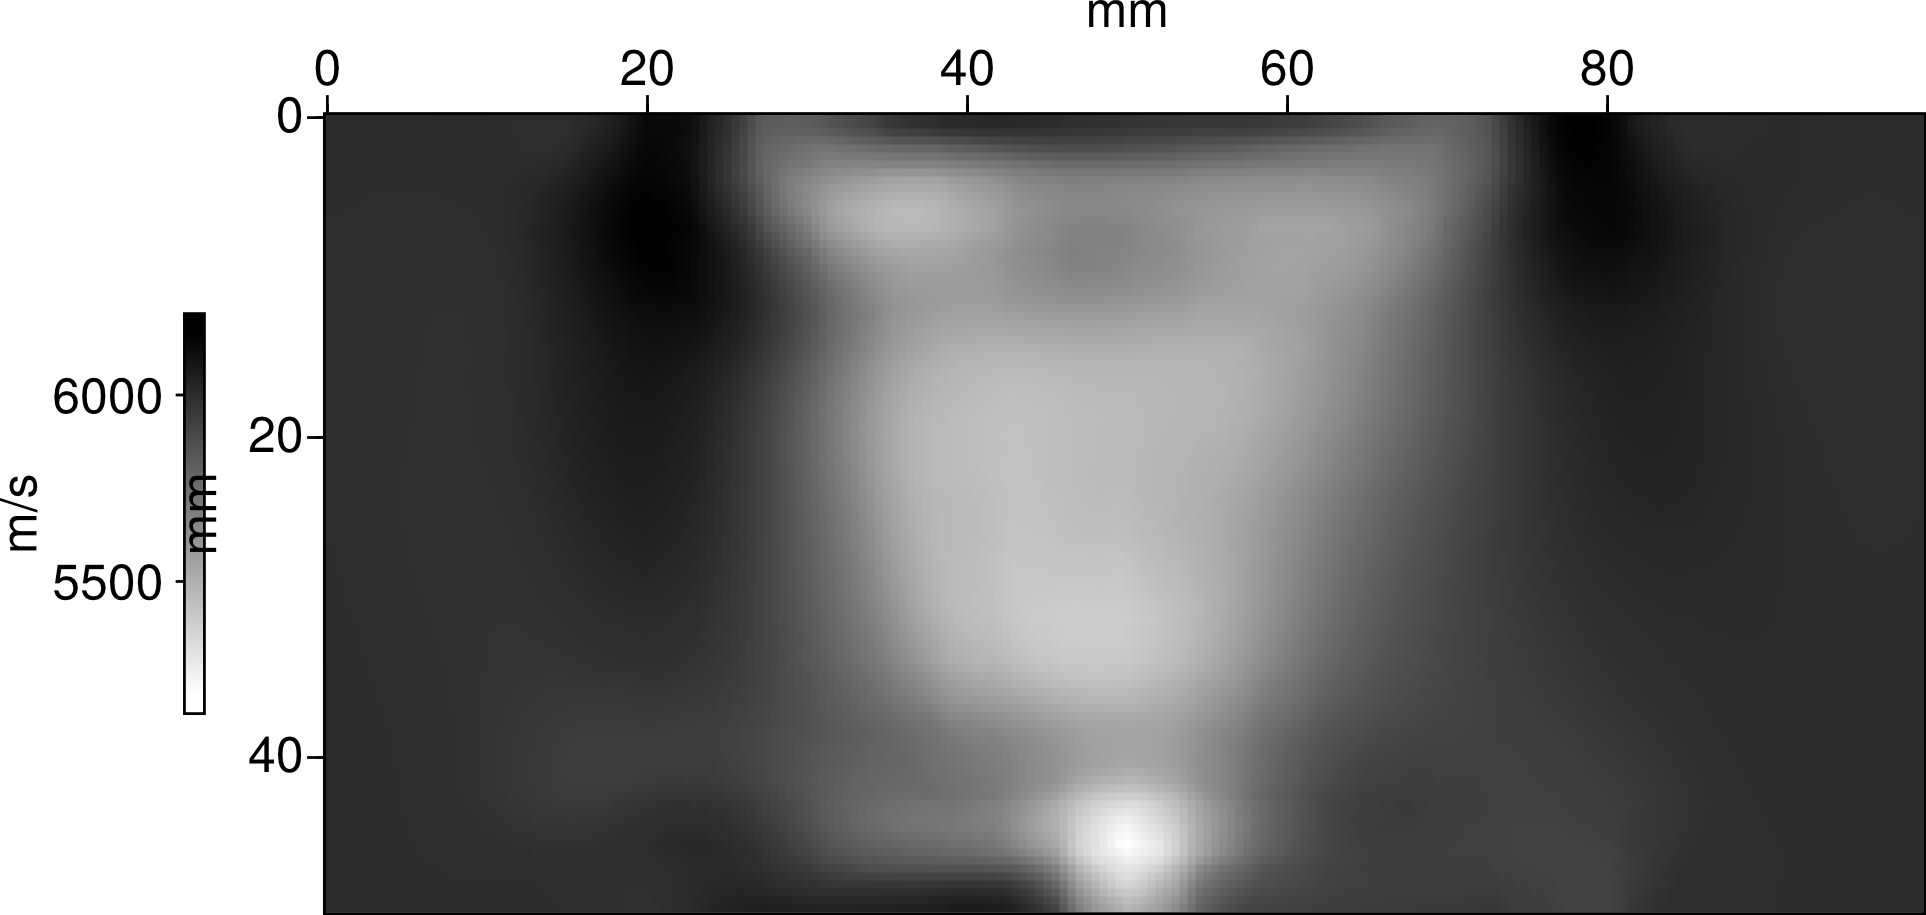
\includegraphics[width=\textwidth]{img/multi_trans/vp_multi_150k.png}
		\end{subfigure}
		\begin{subfigure}[b]{0.23\textwidth}
			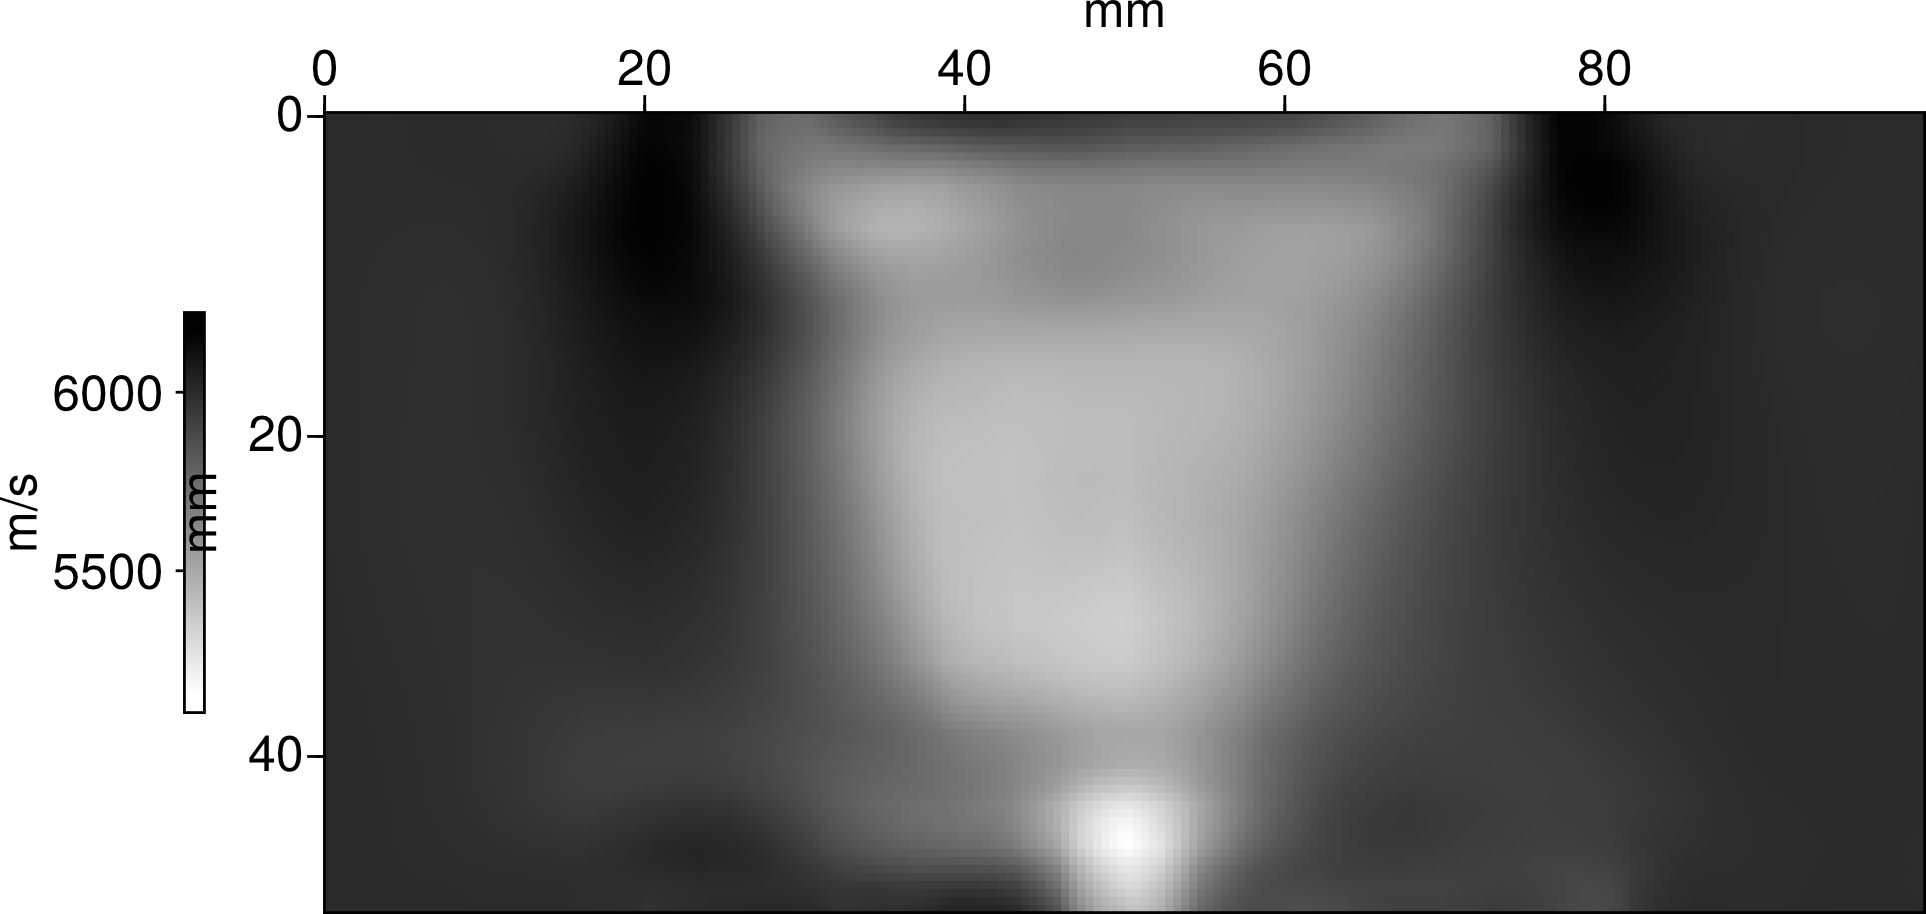
\includegraphics[width=\textwidth]{img/multi_trans/vp_multi_337k.png}
		\end{subfigure}
		\begin{subfigure}[b]{0.23\textwidth}
			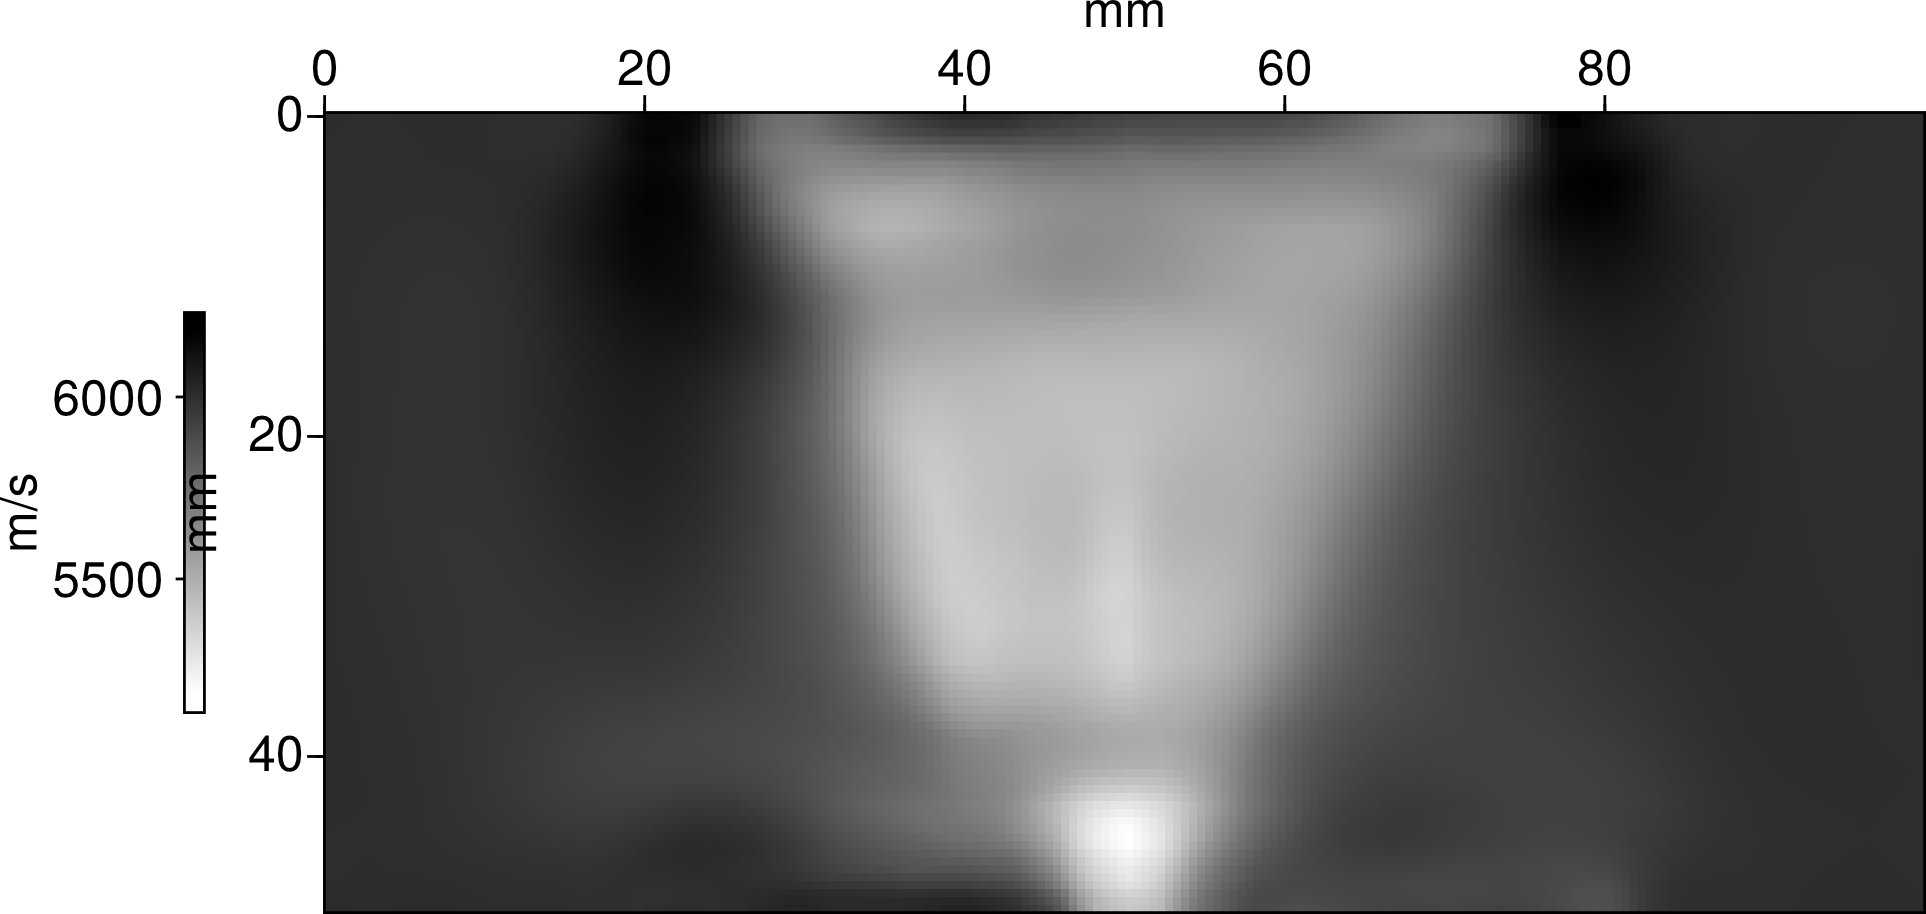
\includegraphics[width=\textwidth]{img/multi_trans/vp_multi_750k.png}
		\end{subfigure}
		\begin{subfigure}[b]{0.23\textwidth}
			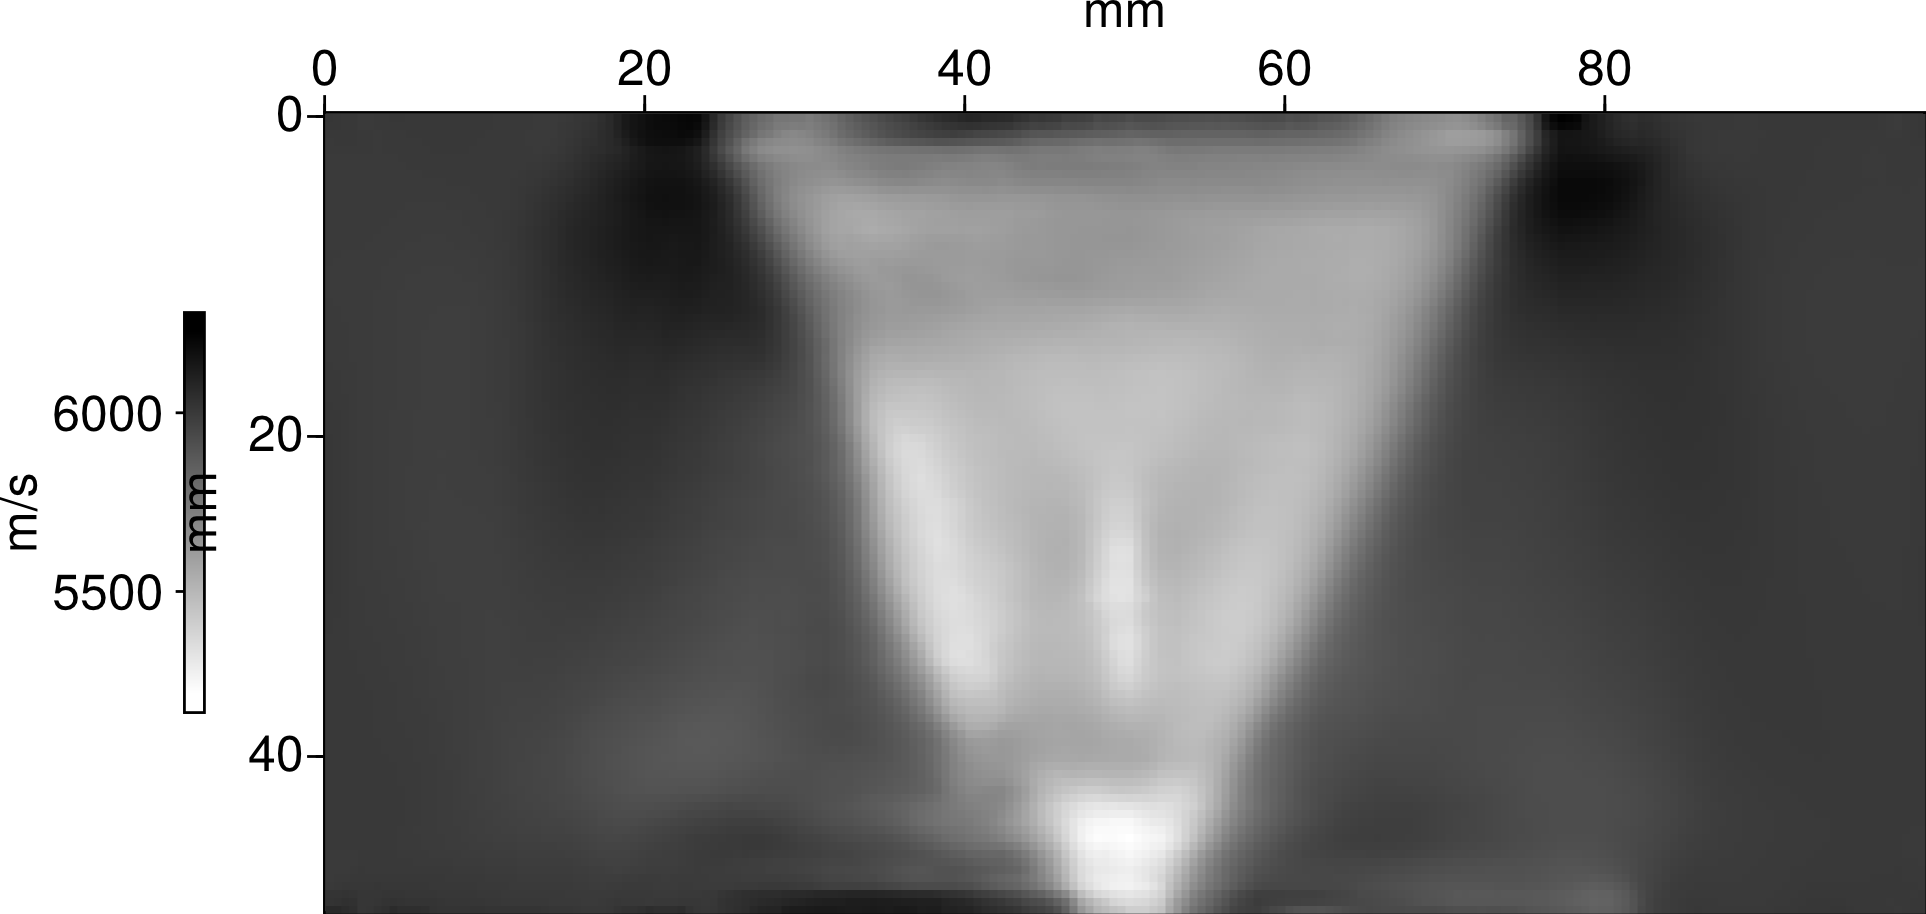
\includegraphics[width=\textwidth]{img/multi_trans/vp_multi_1M.png}
		\end{subfigure}
		
		\begin{subfigure}[b]{0.23\textwidth}
			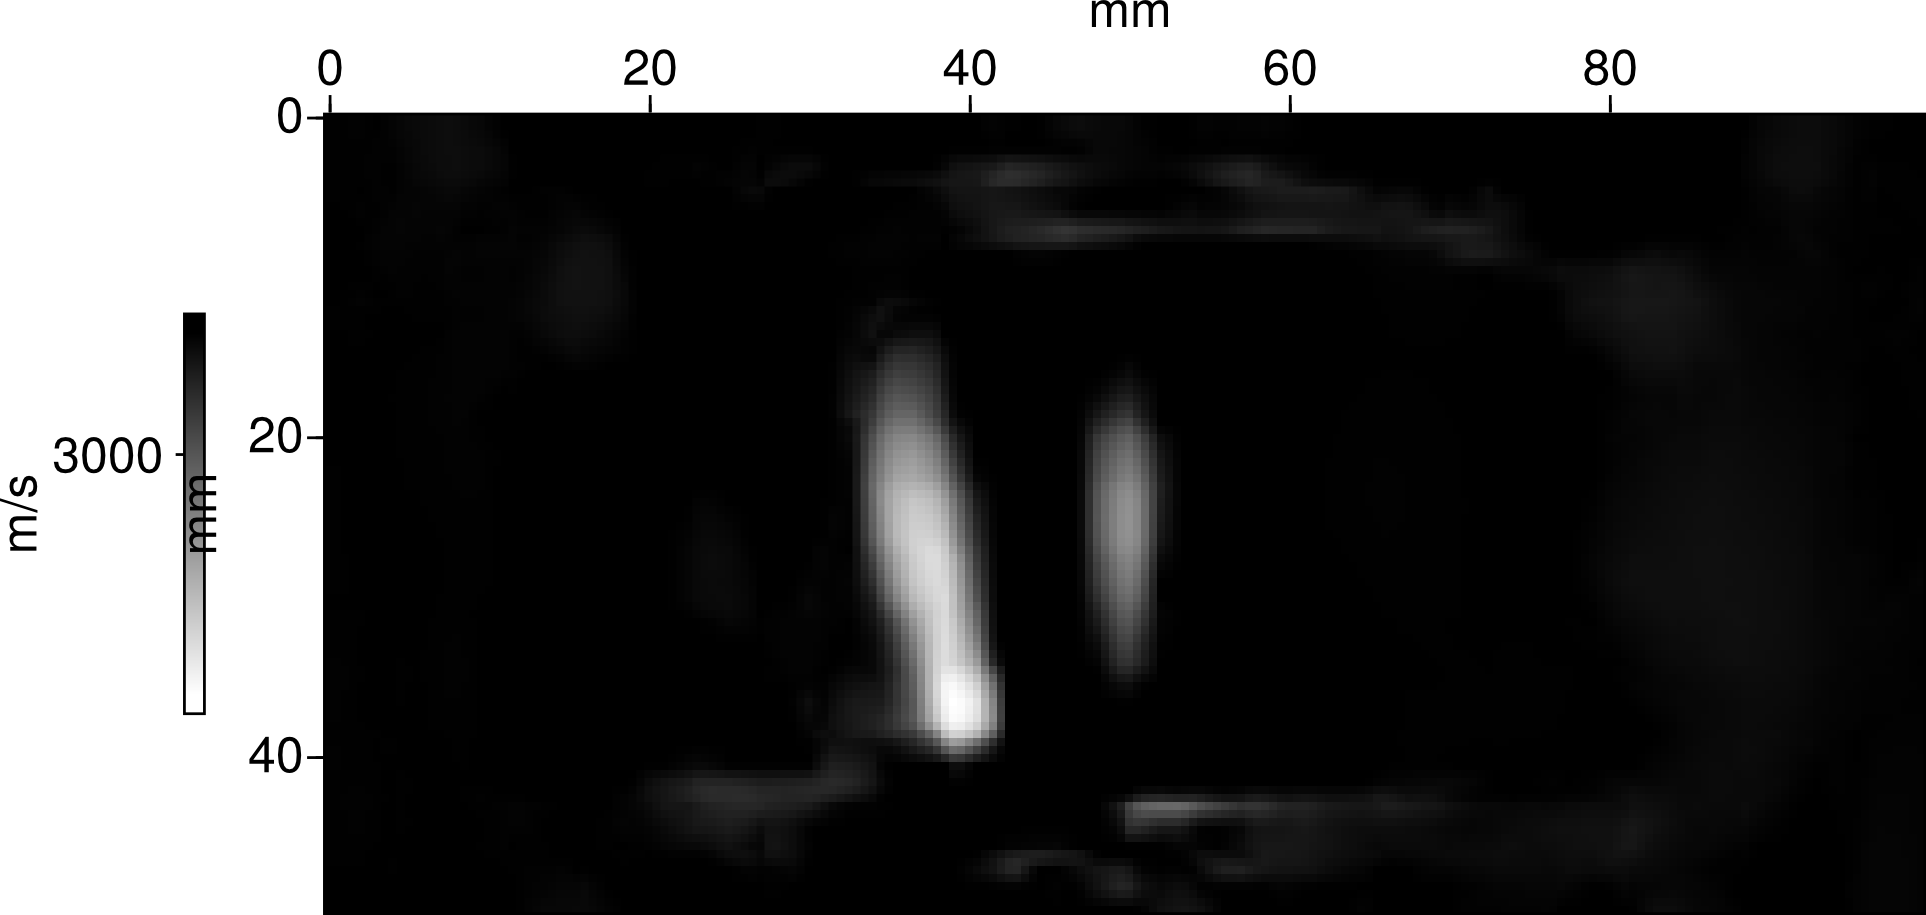
\includegraphics[width=\textwidth]{img/multi_trans/vs_multi_150k.png}
			\caption{150 kHz}
		\end{subfigure}
		\begin{subfigure}[b]{0.23\textwidth}
			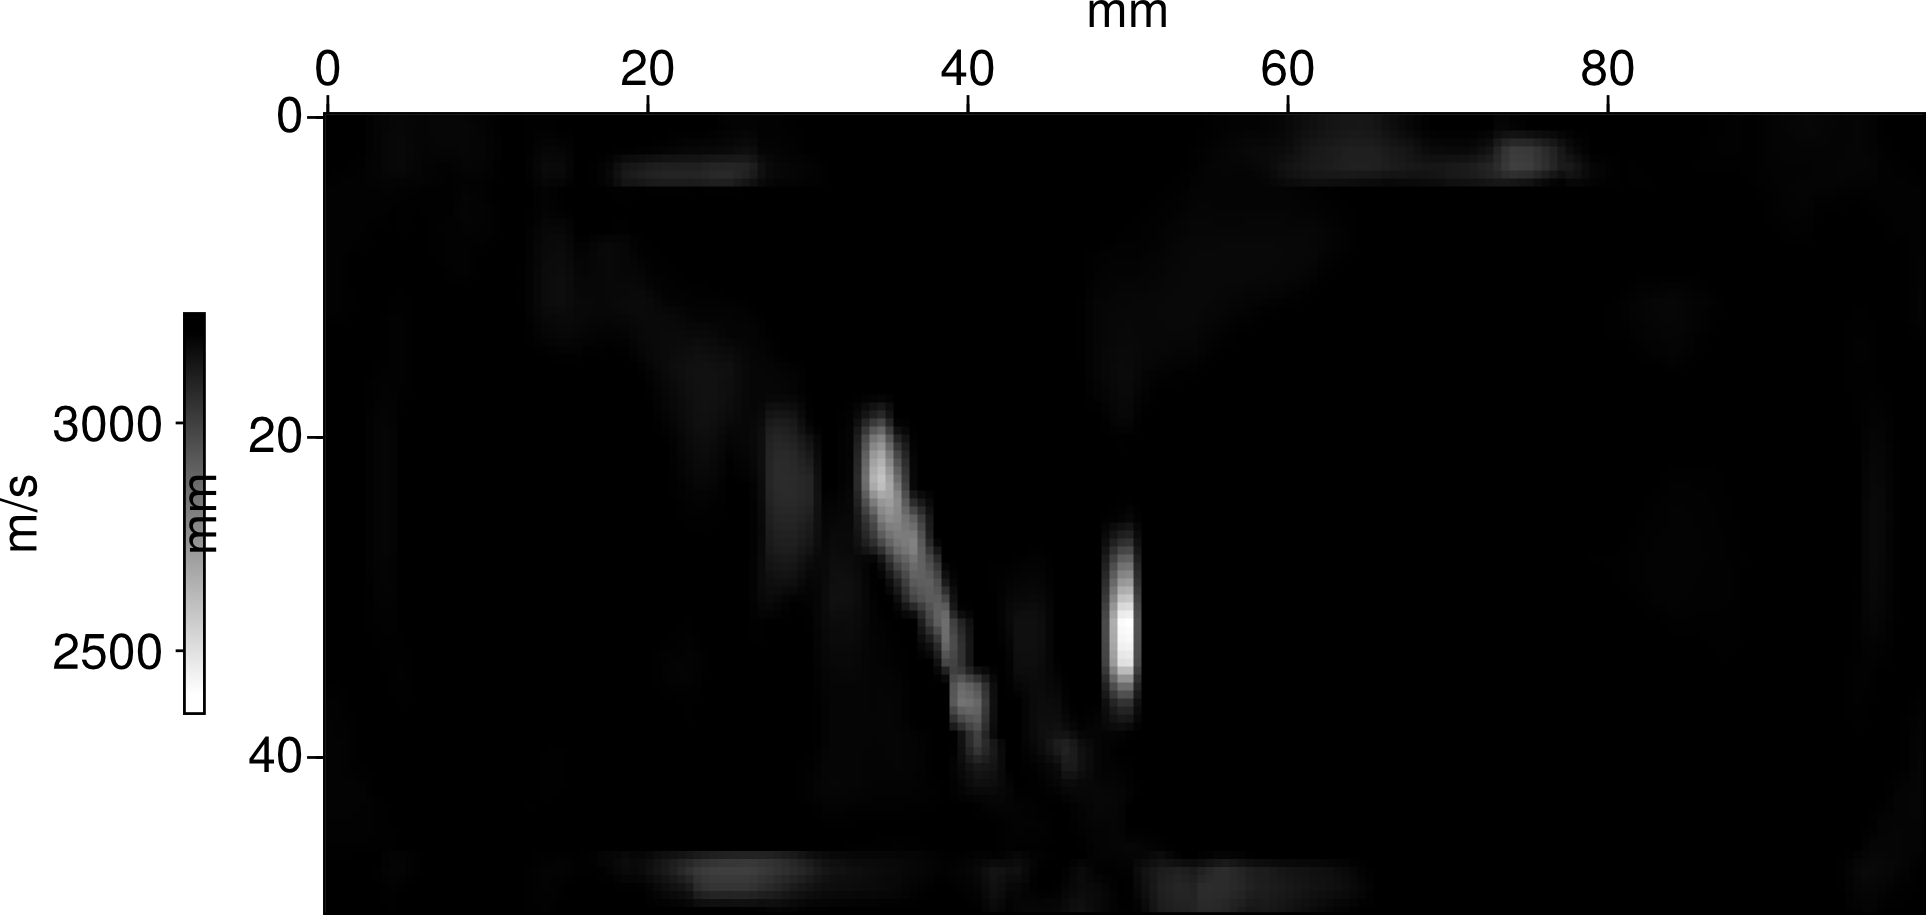
\includegraphics[width=\textwidth]{img/multi_trans/vs_multi_337k.png}
			\caption{337 kHz}
		\end{subfigure}
		\begin{subfigure}[b]{0.23\textwidth}
			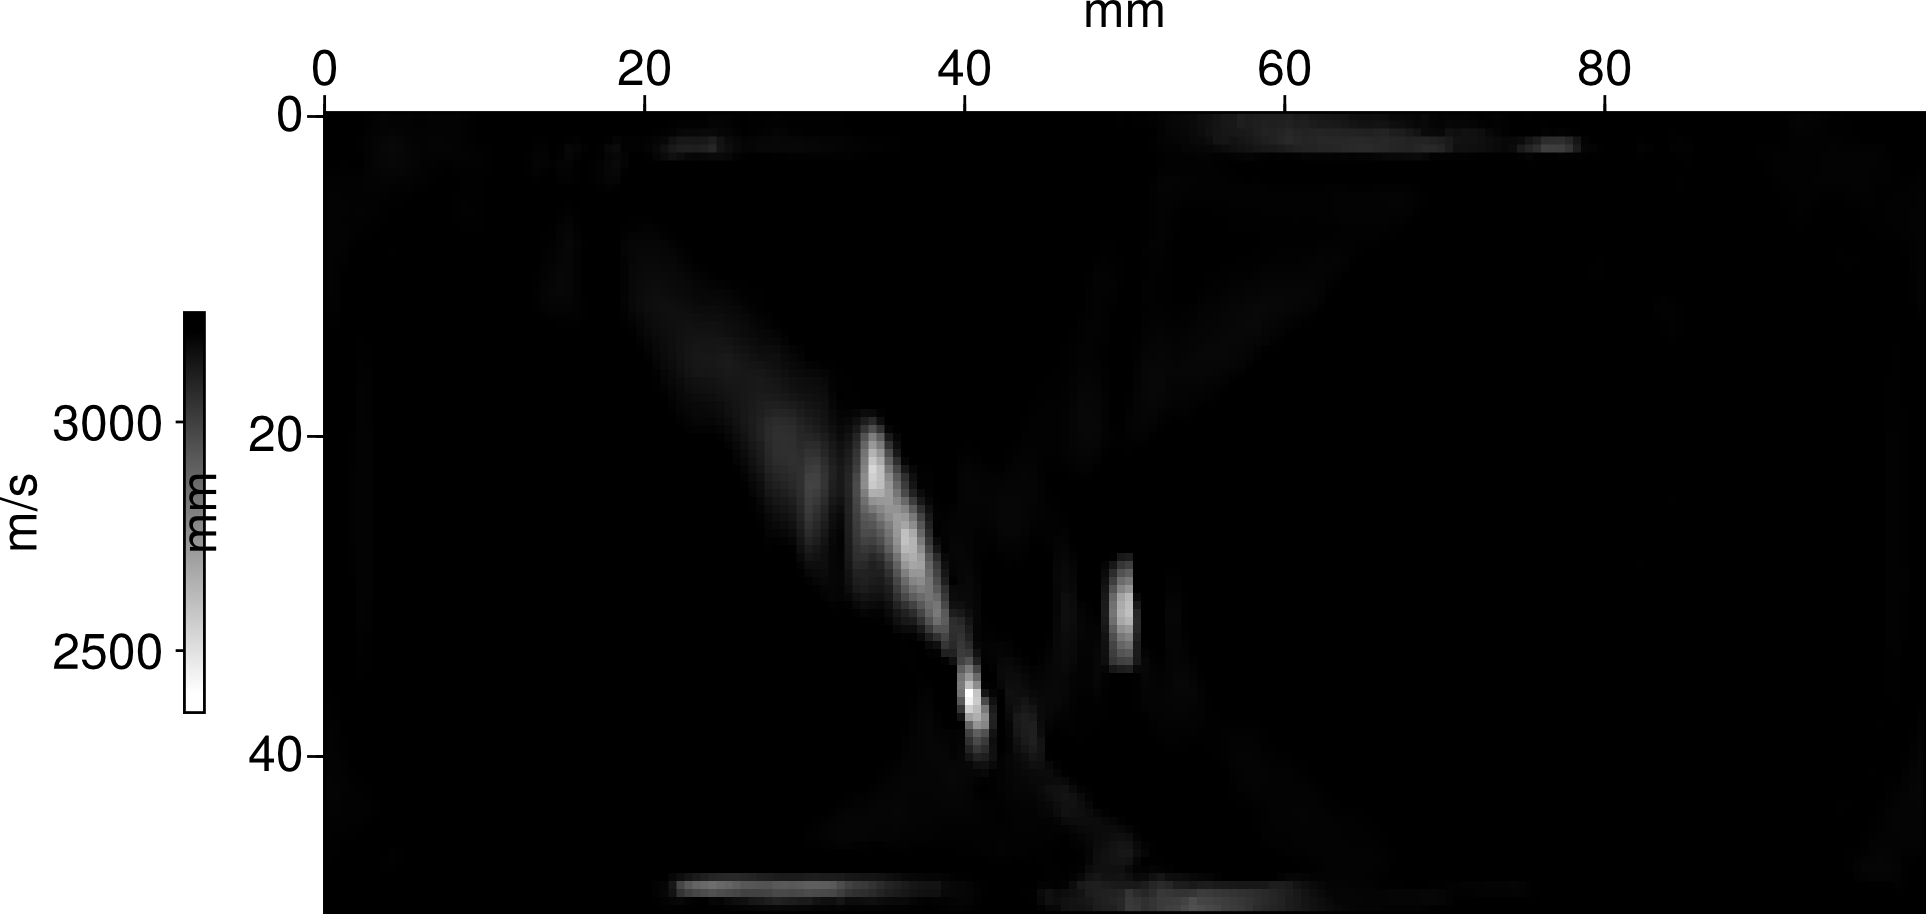
\includegraphics[width=\textwidth]{img/multi_trans/vs_multi_750k.png}
			\caption{750 kHz}
		\end{subfigure}
		\begin{subfigure}[b]{0.23\textwidth}
			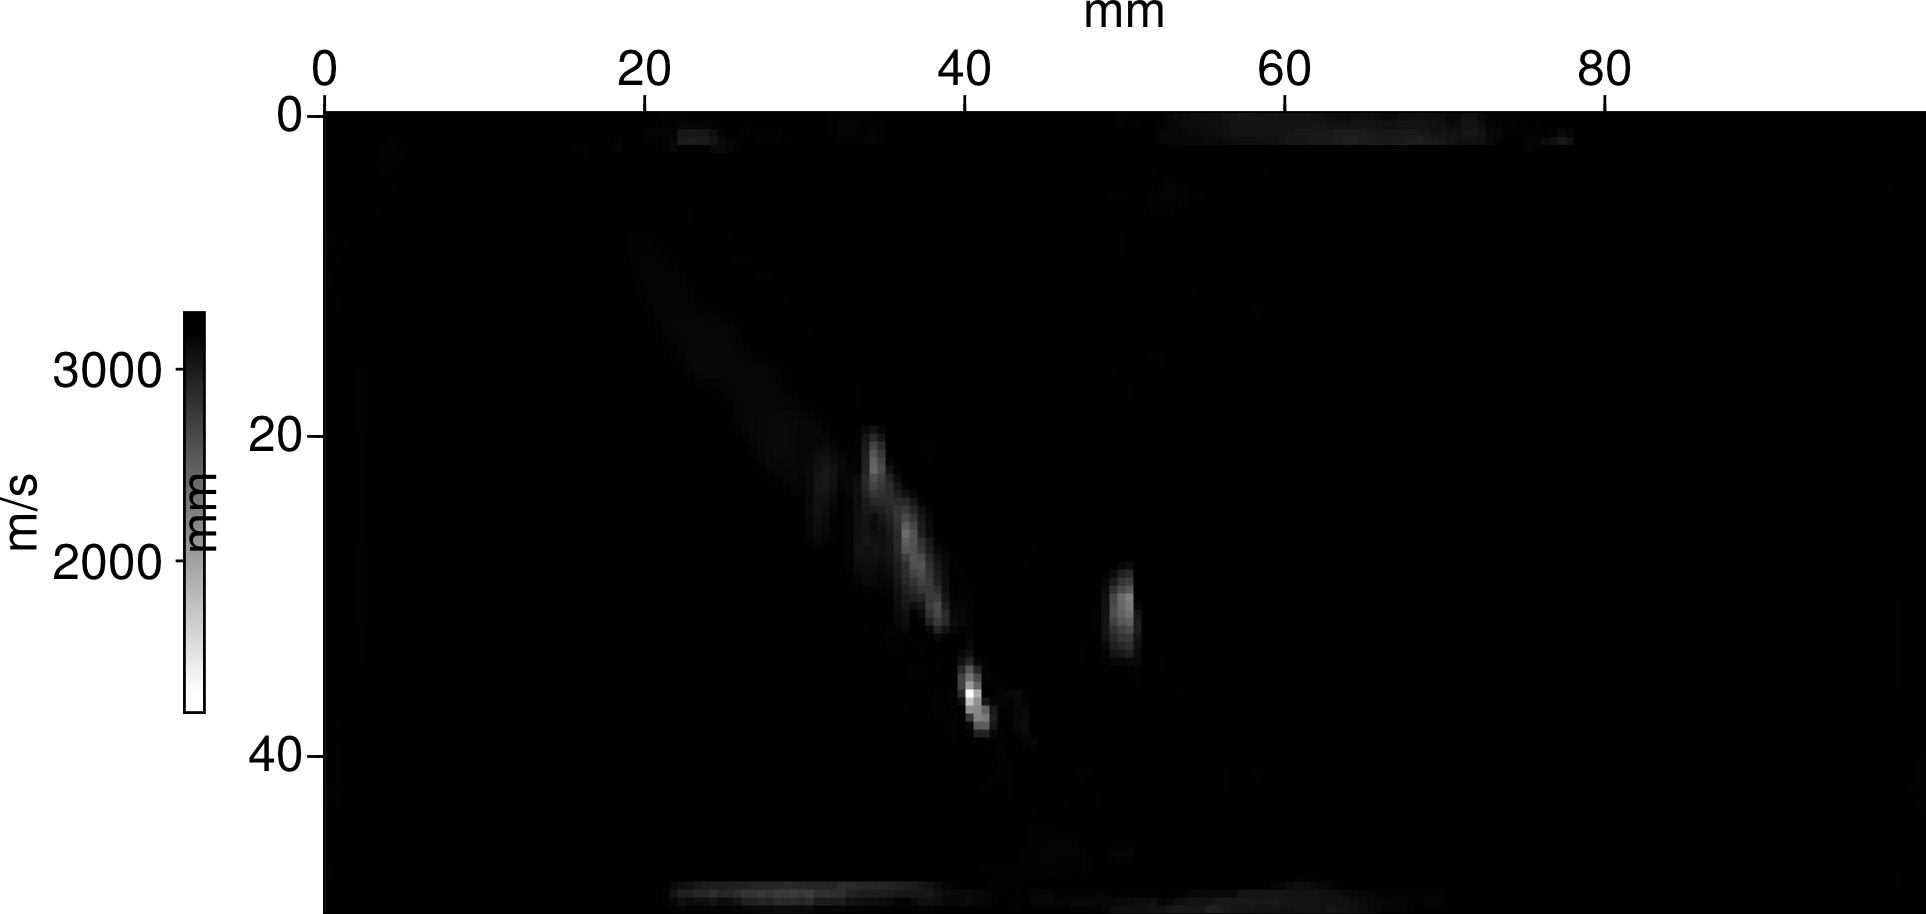
\includegraphics[width=\textwidth]{img/multi_trans/vs_multi_1M.png}
			\caption{1 MHz}
		\end{subfigure}
	\end{changemargin}
	\caption{Résultats d'inversions multiparamètres. En haut : $v_{p}$, en bas : $v_{s}$.\label{res:multi_trans}}
\end{figure}

\begin{figure}[!h]
	\centering
	\begin{subfigure}{0.45\textwidth}
		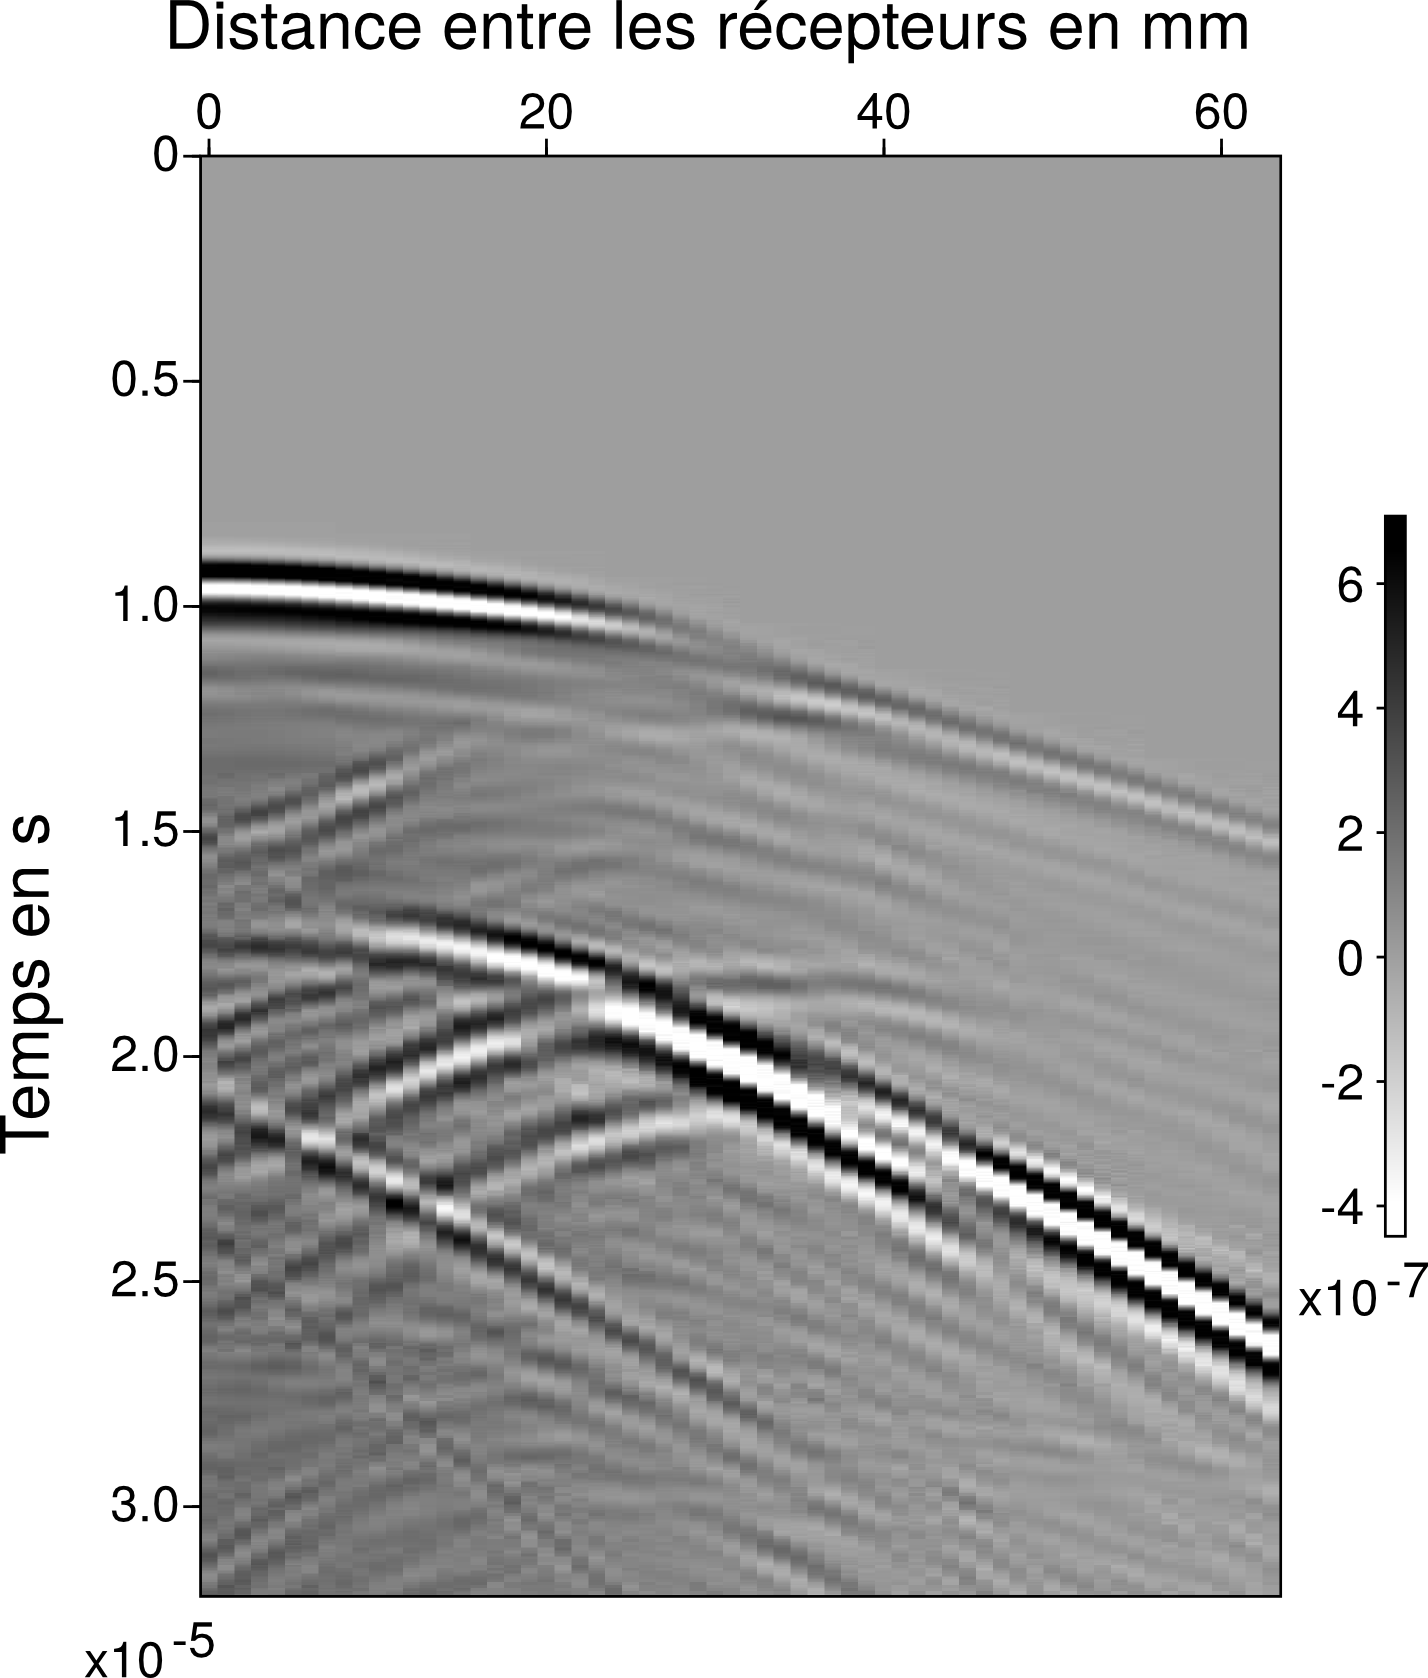
\includegraphics[width=\textwidth]{img/multi_trans/comp/data_true.png}
		\caption{Données de références correspondant à la propagation dans les milieux vrais, à 1MHZ.}
	\end{subfigure}
	\begin{subfigure}{0.45\textwidth}
		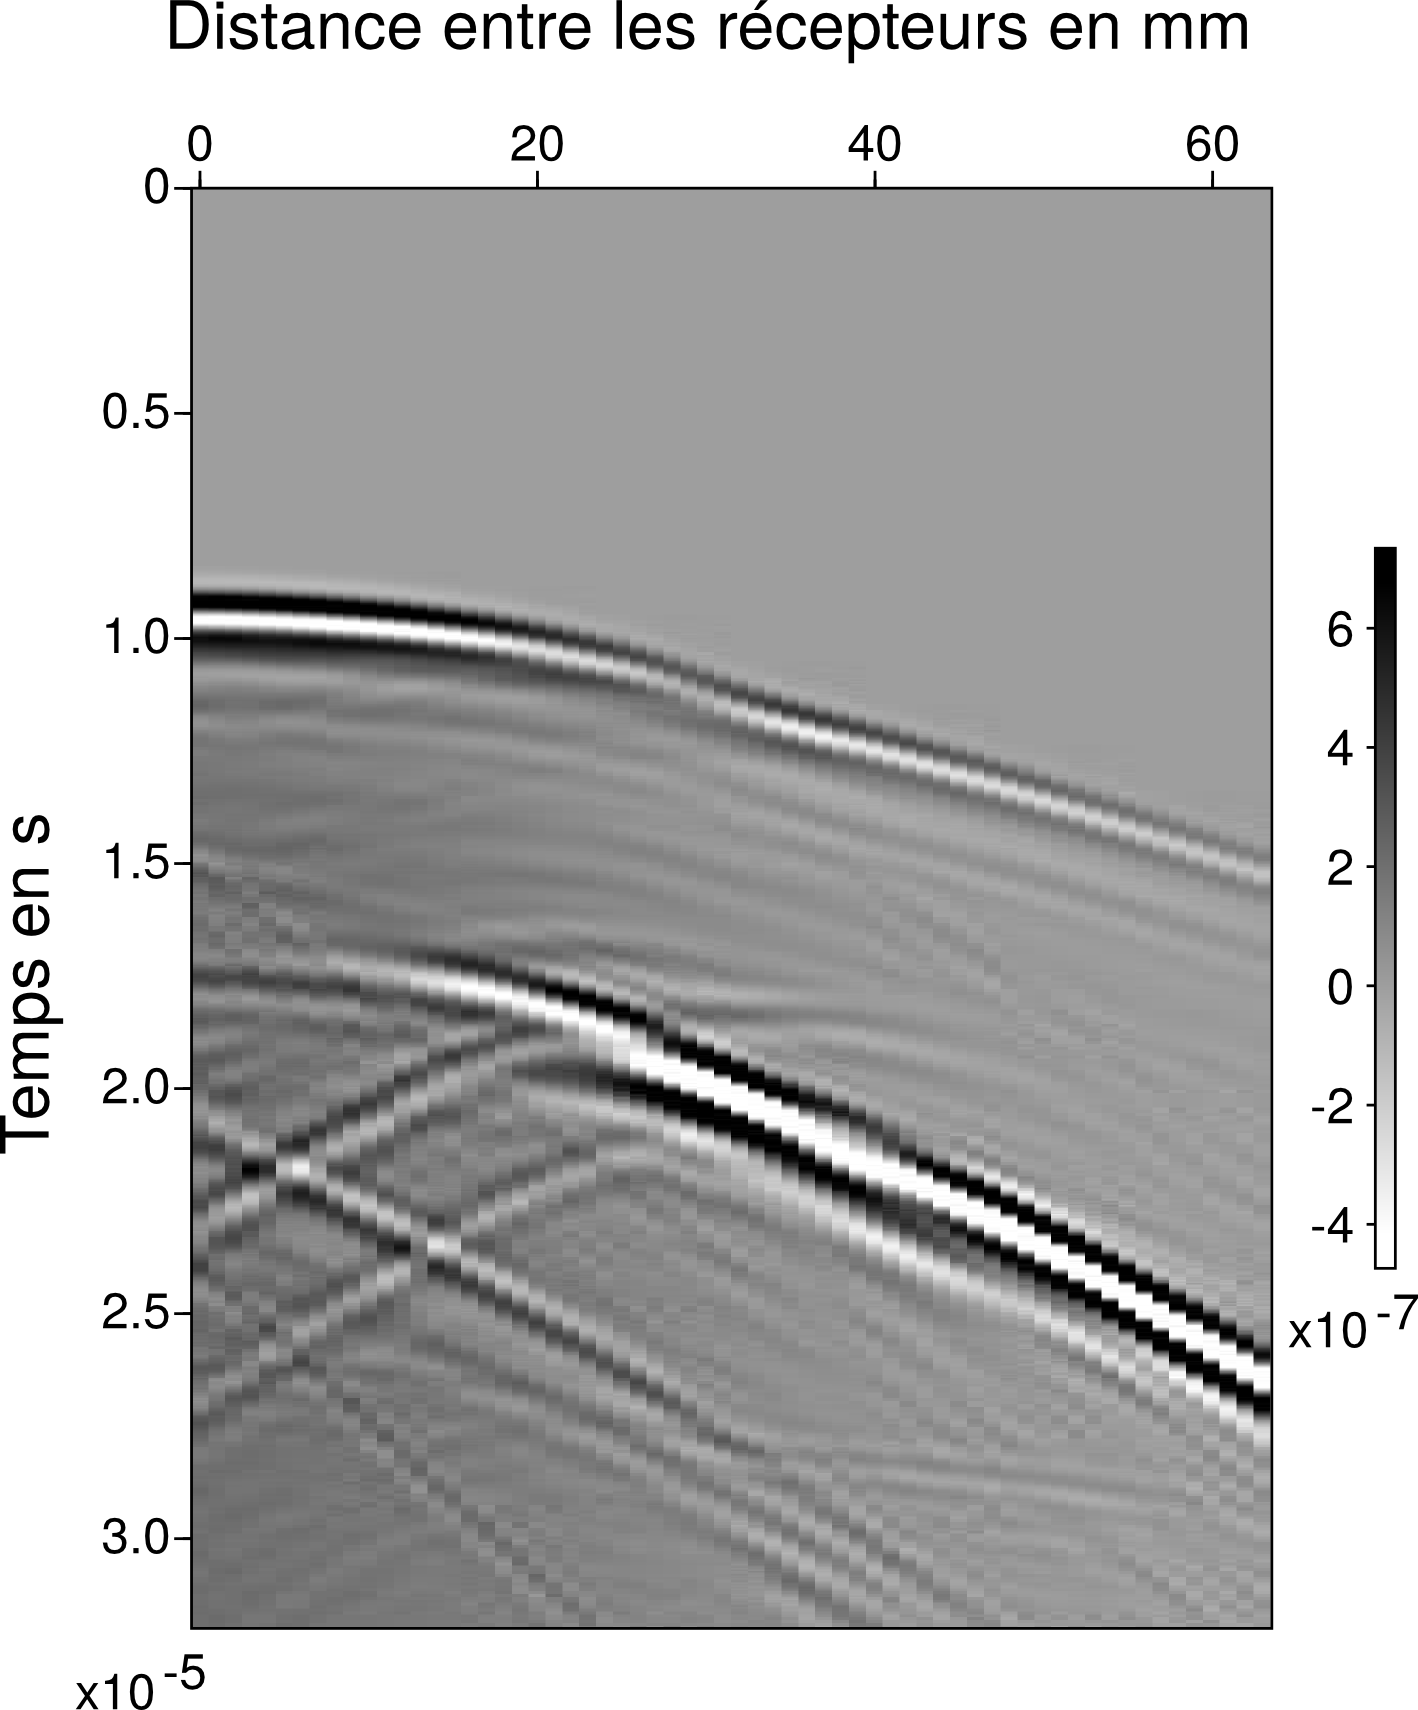
\includegraphics[width=\textwidth]{img/multi_trans/comp/data_built.png}
		\caption{Données issues des milieux reconstruits en dernière inversion, pour une excitation à 1 MHz.}
	\end{subfigure}
	\caption{\label{data1M}}
\end{figure}

\subsection{Résultat d'inversion multiparamètre en réflexion et en transmission}

Afin d'améliorer la reconstruction des nombres d'onde horizontaux, on considère maintenant une acquisition constituée d'une barrette 32 (pour réduction de mémoire) éléments en excitation (placée sur la partie supérieure de la plaque) et de 2 barrettes 64 éléments en réception placées de part et d'autre de la plaque.\\

\subsubsection{Étude des données}
Le milieu vrai est représenté en figure~\ref{config} et les sources y sont repérées en vert. Les distances entre la huitième source et les principaux récepteurs sont représentées et le code couleur est réutilisé pour repérer les différentes réflexions sur les données issues de la huitième source (figure~\ref{data}). Ces données montrent que :
\begin{itemize}
	\item l'onde de surface (visible que sur les données avec surface libre) a une vitesse très proche de celle de l'onde de cisaillement, soit environ 3000 m/s, et est de très forte amplitude,
	\item si les défauts sont suffisamment éloignés des sources, le champ diffracté est principalement mesuré après le passage de l'onde de surface. Un masquage de type \emph{front mute} semble donc plus indiqué qu'un \emph{tail mute},
	\item la réflexion sur le bord absorbant gauche (onde verte) est d'amplitude importante et n'est pas masqué par le \emph{front mute} délimité par la ligne tiretée.
\end{itemize}


\paragraph{Note}  Un masque est appliqué sur les données acquise par la barrette du haut uniquement. Pour cela, il faut ajouter à la fonction \emph{compute\_weight\_data.f90} une condition sur l'application du masque du type : 
\begin{verbatim}
    if(ABS((acqui%s1(isrc)-acqui%r1(irec)))< X ) THEN 
        application du masque
    end if
\end{verbatim}
où \texttt{acqui\%s1(isrc)} est la position de la source \texttt{isrc} en z et \texttt{acqui\%r1(irec)} est la position du recepteur \texttt{irec} en z. Le masque n'est ainsi pas appliqué pour un écart en z supérieur à \texttt{X} entre source et récepteur d'un couple considéré.


Pour que l'onde de surface et ses réflexions sur les bords absorbants soient correctement filtré, sans perdre trop d'information contenues dans les réflexions sur les défauts, un filtre fk semble plus approprié qu'un masque des données temporelles.



\begin{figure}[!h]
	\centering
	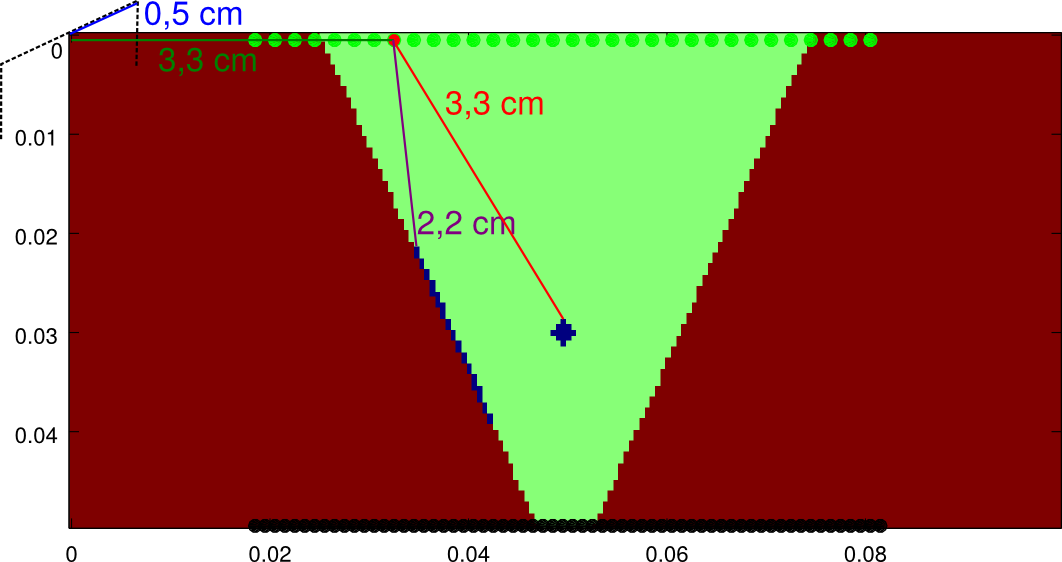
\includegraphics[height=5cm]{img/multi_ref_trans/config.png}
	\caption{Configuration du système d'acquisition  : les disques noirs sont les récepteurs de la barrette du bas (celle du haut n'est pas représentée) et les cercles verts sont les sources. Les distances entre la huitième source et quelques principaux réflecteurs sont indiquées.\label{config}}
\end{figure}

\begin{figure}[!h]
	\centering
	\begin{subfigure}{0.45\textwidth}
		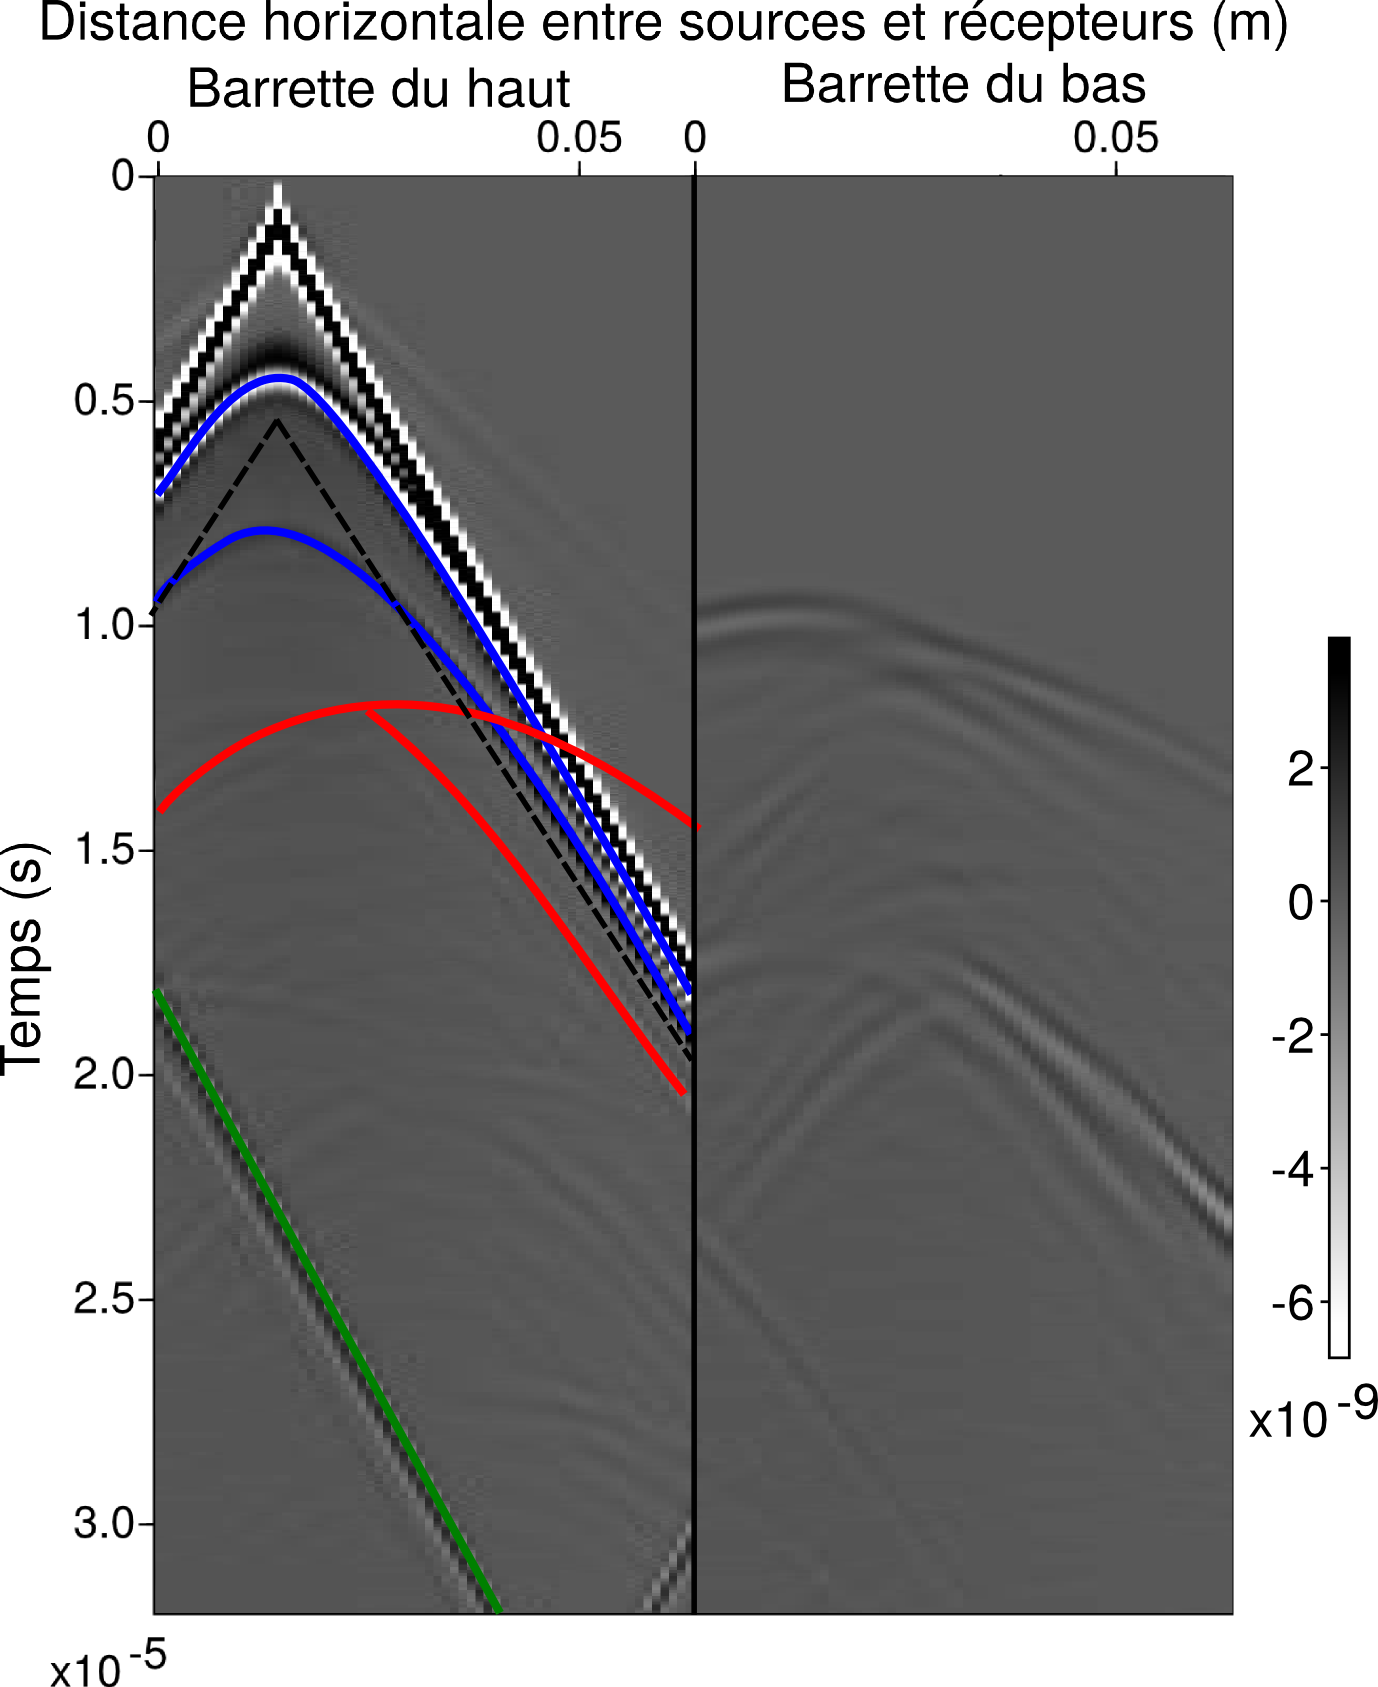
\includegraphics[width=\textwidth]{img/multi_ref_trans/data_2freesurf.png}
		\caption{Données observées pour une excitation à 1 MHz dans le milieu comportant deux surfaces libres.}
	\end{subfigure}
	\begin{subfigure}{0.45\textwidth}
		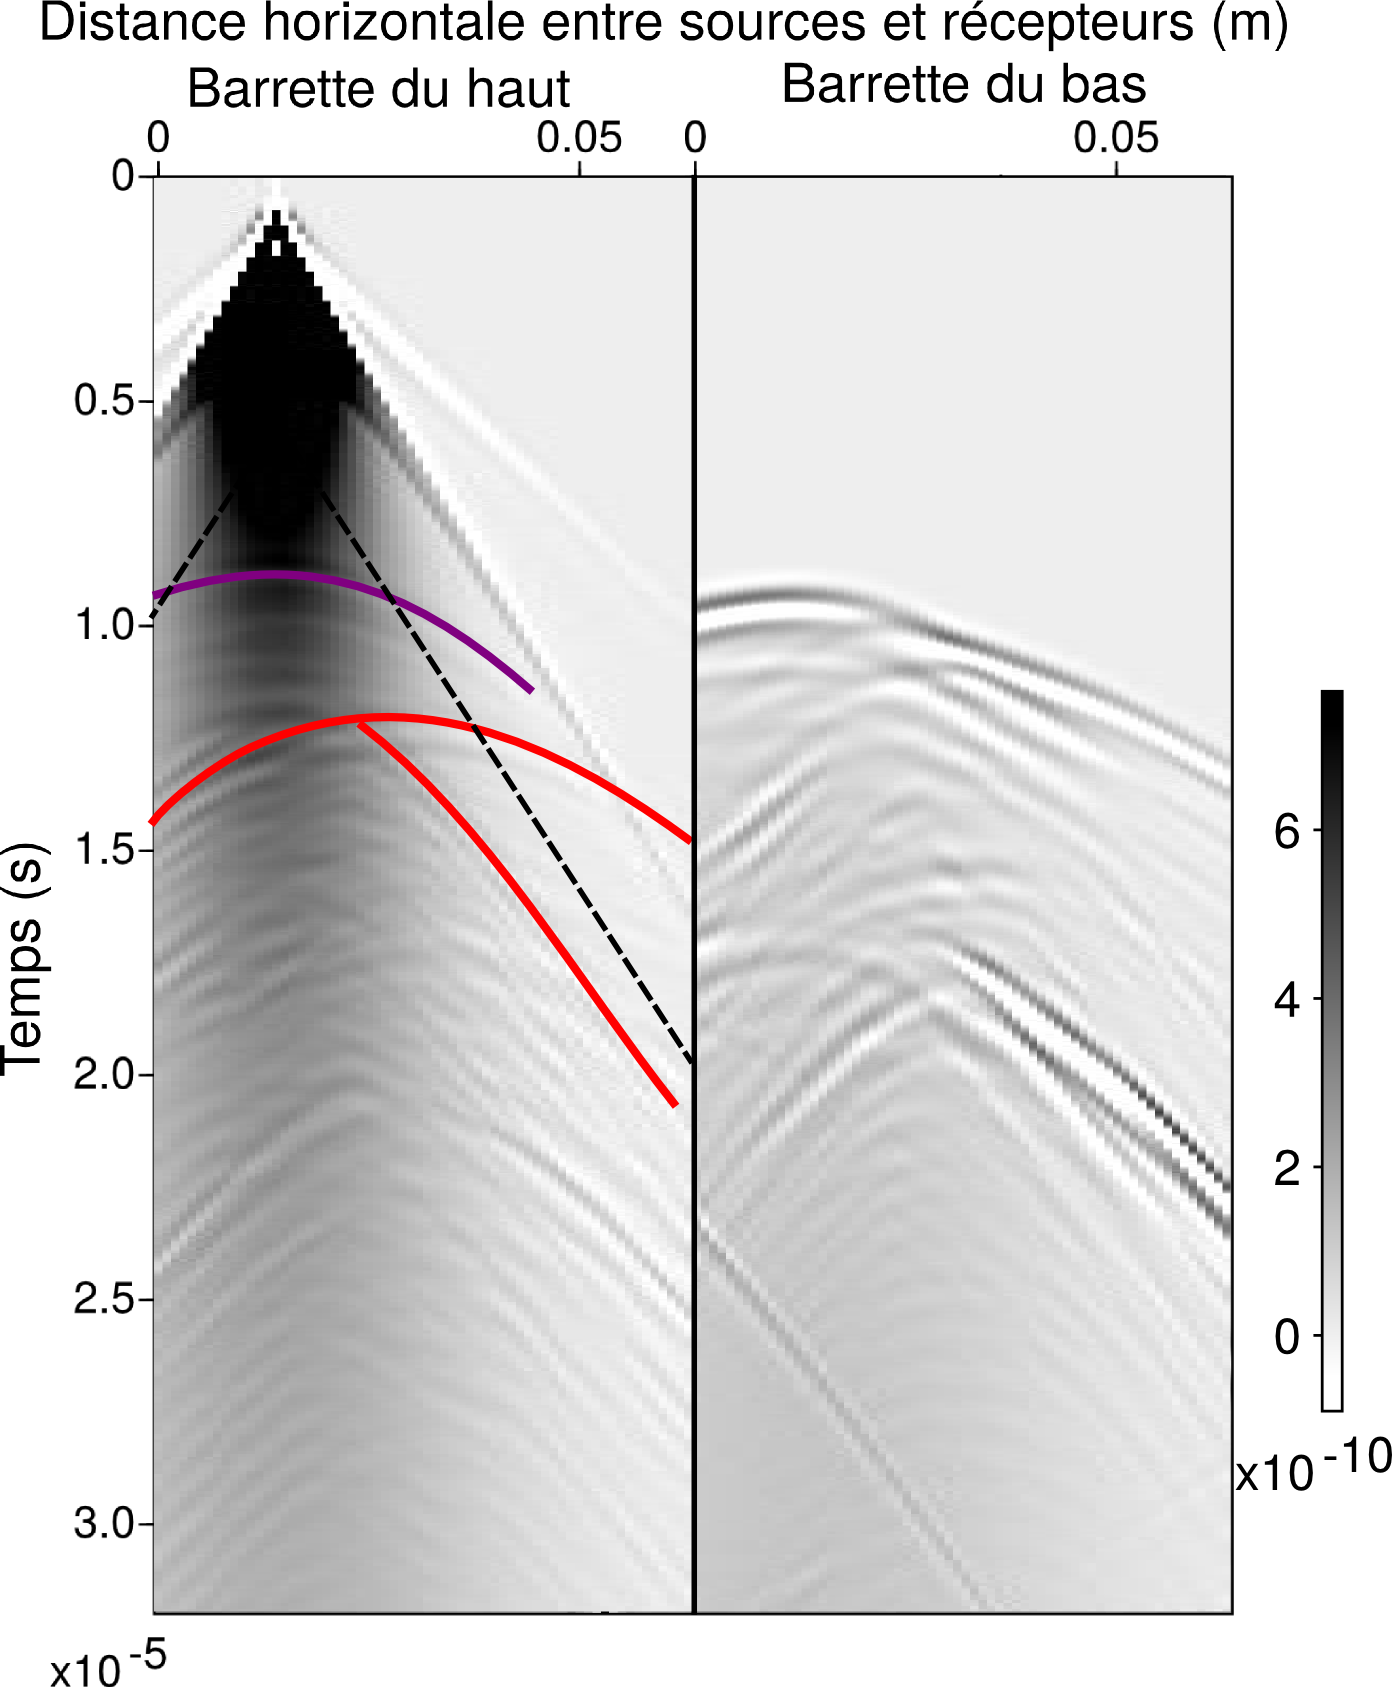
\includegraphics[width=\textwidth]{img/multi_ref_trans/data_0freesurf.png}
	\caption{Données observées pour une excitation à 1 MHz dans le milieu sans surface libre.\\~}
	\end{subfigure}
	\caption{Données observées pour une excitation par la huitième source.\\
	Ondes bleues : réflexions de l'onde de surface dans les bords absorbants situés dans le plan (xz),\\
	Ondes rouges : réflexion P et S de l'onde P sur l'inclusion,\\
	Onde violette : réflexion sur la partie supérieure de la fissure,\\
	Onde verte : réflexion de l'onde de surface sur le bord absorbant gauche situé dans le plan (zy).
	La ligne tiretée indique une possibilité de masquage des données antérieures à cette ligne.\label{data}}
\end{figure}

%image données masquées avec le masque qui fonctionne

%onde de surface lente = très petite longueur d'onde = prendre un maillage plus fin


\end{document} % fin doc


